%%%%%%%%%%%%%%%%%%%%%%%%%%%%%%%%%%%%%%%%%%%%%%%%%%%%%%%%%%%%%%%%%%%%%%%%%%%%%%%%%%%%%%%%%%%%%%%%%%%%%%%%%%%%%%%%%%%%%%%%%%%%%%%%%%%%%%%%%%%%%%%%%%%%%%%%%%%
% This is just an example/guide for you to refer to when submitting manuscripts to Frontiers, it is not mandatory to use Frontiers .cls files nor frontiers.tex  %
% This will only generate the Manuscript, the final article will be typeset by Frontiers after acceptance.   
%                                              %
%                                                                                                                                                         %
% When submitting your files, remember to upload this *tex file, the pdf generated with it, the *bib file (if bibliography is not within the *tex) and all the figures.
%%%%%%%%%%%%%%%%%%%%%%%%%%%%%%%%%%%%%%%%%%%%%%%%%%%%%%%%%%%%%%%%%%%%%%%%%%%%%%%%%%%%%%%%%%%%%%%%%%%%%%%%%%%%%%%%%%%%%%%%%%%%%%%%%%%%%%%%%%%%%%%%%%%%%%%%%%%

%%% Version 3.4 Generated 2022/06/14 %%%
%%% You will need to have the following packages installed: datetime, fmtcount, etoolbox, fcprefix, which are normally inlcuded in WinEdt. %%%
%%% In http://www.ctan.org/ you can find the packages and how to install them, if necessary. %%%
%%%  NB logo1.jpg is required in the path in order to correctly compile front page header %%%

\documentclass[utf8]{FrontiersinHarvard} % for articles in journals using the Harvard Referencing Style (Author-Date), for Frontiers Reference Styles by Journal: https://zendesk.frontiersin.org/hc/en-us/articles/360017860337-Frontiers-Reference-Styles-by-Journal
%\documentclass[utf8]{FrontiersinVancouver} % for articles in journals using the Vancouver Reference Style (Numbered), for Frontiers Reference Styles by Journal: https://zendesk.frontiersin.org/hc/en-us/articles/360017860337-Frontiers-Reference-Styles-by-Journal
%\documentclass[utf8]{frontiersinFPHY_FAMS} % Vancouver Reference Style (Numbered) for articles in the journals "Frontiers in Physics" and "Frontiers in Applied Mathematics and Statistics" 

%\setcitestyle{square} % for articles in the journals "Frontiers in Physics" and "Frontiers in Applied Mathematics and Statistics" 
\usepackage{url,hyperref,lineno,microtype,subcaption,caption}
\usepackage[onehalfspacing]{setspace}
\usepackage{algorithm}
\usepackage{algorithmic}
\usepackage{graphicx}
% Project figures/ at repo root (e.g., prism.openai.com: use workspace root as the build directory).
% Also resolves when running pdflatex from Paper/ or Paper/frontiers/.
\graphicspath{{./figures/}{../figures/}{../../figures/}}
\usepackage[section]{placeins}
\usepackage{textcomp}
\usepackage{soul}
\sethlcolor{blue}
\usepackage[table]{xcolor}
\usepackage{multirow}
\usepackage[utf8]{inputenc}
\usepackage{booktabs}
\usepackage{tikz}
\usepackage[dvipsnames]{xcolor}
\usepackage{pgfplots}
\usetikzlibrary{shapes.geometric,arrows,positioning}
\pgfplotsset{compat=1.18}

\linenumbers


% Leave a blank line between paragraphs instead of using \\


\def\keyFont{\fontsize{8}{11}\helveticabold }
\def\firstAuthorLast{Sreevallabh {et~al.}} %use et al only if is more than 1 author
\def\Authors{Kakarala Sreevallabh\,$^{1}$, Kothapalli Anusha\,$^{1}$, Ayesha Shaik\,$^{2, *}$ and Ananthakrishnan Balasundaram \,$^{2}}
% Affiliations should be keyed to the author's name with superscript numbers and be listed as follows: Laboratory, Institute, Department, Organization, City, State abbreviation (USA, Canada, Australia), and Country (without detailed address information such as city zip codes or street names).
% If one of the authors has a change of address, list the new address below the correspondence details using a superscript symbol and use the same symbol to indicate the author in the author list.

\def\Address{$^{1}$School of Computer Science, Vellore Institute of Technology, Chennai, India\\
$^{2}$Centre for Cyber Physical Systems, Vellore Institute of Technology, Chennai, India}
% The Corresponding Author should be marked with an asterisk
% Provide the exact contact address (this time including street name and city zip code) and email of the corresponding author
\def\corrAuthor{Ayesha Shaik}

\def\corrEmail{ayesha.sk@vit.ac.in}

\begin{document}
\onecolumn
\firstpage{1}

\title[Cross-Modal Knowledge Transfer]{Cross-Modal Knowledge Transfer for Cost-Effective Mango Disease Detection Using Synthetic Thermal Imaging} 

\author[\firstAuthorLast ]{\Authors} %This field will be automatically populated
\address{} %This field will be automatically populated
\correspondance{} %This field will be automatically populated

\extraAuth{}% If there are more than 1 corresponding author, comment this line and uncomment the next one.
%\extraAuth{corresponding Author2 \\ Laboratory X2, Institute X2, Department X2, Organization X2, Street X2, City X2 , State XX2 (only USA, Canada and Australia), Zip Code2, X2 Country X2, email2@uni2.edu}


\maketitle

\begin{abstract}

%%% Leave the Abstract empty if your article does not require one, please see the Summary Table for full details.
\section{}
Thermal cameras play a crucial role in identifying diseases invisible to regular photographs, but they are prohibitively expensive for many orchards to purchase (typically exceeding $25,000$). The proposed work study to what extent the advantages of the thermal signal can be approximated using only RGB data. The proposed method trains a supervised lesion detector on a leaf pathology dataset (MangoLeafBD) to learn universal disease manifestation patterns. These learned lesion features are transferred to fruit images and transformed into synthetic thermal-like maps through a physics-informed model that simulates metabolic heat signatures. The synthetic thermal maps are then fused with the original RGB features via a 16-head multi-head attention mechanism that automatically weights disease-relevant cues from both modalities. In the case of mango disease recognition across five classes, the system attains an accuracy of 87.3\%, which is a 4.8\% gain over the best RGB-only baseline (RGB ViT-Base at 85.8\%), without involving any additional hardware. The proposed method achieves approximately 89\% of the performance of a real thermal camera system (93.5\%) while incurring zero hardware cost compared to \$25,000 for thermal cameras or \$50,000 for multi-spectral systems, making it directly deployable on commodity smartphones for low-cost crop health monitoring.

\tiny
 \keyFont{ \section{Keywords:} cross-modal learning, mango disease detection, thermal simulation, knowledge transfer, precision agriculture, attention-based fusion, deep learning} %All article types: you may provide up to 8 keywords; at least 5 are mandatory.
\end{abstract}
\section{Introduction}

Crop diseases remain one of the most persistent threats to global food security, with annual losses estimated at 10--16\% of global harvest value \cite{fao2021,fao2023,savary2019}. Mango (\textit{Mangifera indica}), the fifth most produced fruit crop worldwide, is particularly vulnerable to diseases such as anthracnose, alternaria, black mould rot, and stem-end rot, which can spread rapidly through orchards and devastate yields if not detected early \cite{singh2019}. Timely and accurate disease diagnosis is therefore critical for effective crop management and economic sustainability.

In recent years, deep learning has emerged as a powerful tool for automated plant disease detection from images \cite{mohanty2016,ferentinos2018,thakur2022}. Convolutional neural networks (CNNs) trained on RGB photographs can classify diseases in real time on smartphones, offering a low-cost alternative to laboratory analysis \cite{kamilaris2018,coulibaly2022}. However, RGB-only approaches typically achieve accuracies between 75--85\% and struggle with diseases that manifest primarily through internal tissue changes not visible on the surface \cite{pineda2021,abade2021}. Recent comprehensive reviews have highlighted that while deep learning models continue to improve in accuracy, the reliance on a single imaging modality remains a fundamental bottleneck \cite{thakur2022,hasan2024}.

Multi-modal imaging, particularly the combination of RGB with thermal sensing, has shown significant promise for improving detection accuracy \cite{khanal2017,maimaitijiang2020}. Thermal cameras detect temperature variations caused by metabolic stress in diseased tissue, providing complementary information that is invisible to standard cameras \cite{mahlein2016,pineda2021}. Infected regions typically exhibit temperature elevations of 2--5$^{\circ}$C above healthy tissue baselines due to cell lysis and altered transpiration \cite{mahlein2016}. Despite these advantages, thermal imaging equipment costs typically exceed \$25,000, placing multi-modal solutions beyond the reach of smallholder farmers who produce the majority of the world's mangoes \cite{sishodia2020}.

Existing diagnostic methods all come with serious limitations. Expert field diagnosis costs little, but it's slow, relies on personal judgment, and only reaches 65–75\% accuracy in reports \cite{ferentinos2018}. Lab tests deliver strong sensitivity (90–95\%), though they rack up big expenses and long waits that block quick action \cite{martinelli2015}. Deep learning on RGB images works in real time on phones for next to nothing, but it doesn't match the performance of systems that incorporate thermal imaging \cite{mohanty2016,hasan2024}. Recent work on knowledge distillation \cite{hinton2015,li2023_kd} and cross-modal learning \cite{xu2023} suggests that it may be possible to transfer knowledge between modalities without requiring both modalities at inference time, but these techniques have not been applied to the specific problem of simulating thermal information from RGB in agricultural contexts.

This paper addresses a practical question: can we approximate the diagnostic advantages of thermal imaging using only RGB data by learning from related plant anatomy? We propose a cross-modal knowledge transfer framework that borrows disease cues learned from leaf pathology images to generate synthetic thermal-like representations for fruit images, which are then fused with RGB features via an attention-based mechanism. The contributions of the proposed work are as follows:

\begin{itemize}
    \item A cross-domain transfer strategy that leverages leaf lesion patterns to infer thermal cues in fruit imagery.
    \item A physics-informed approach for generating thermal-like maps from lesion probabilities.
    
    \item A fusion module using multi-head attention (16 heads) to blend RGB and synthetic thermal features, including learned gating that dynamically adjusts the weight of each modality.
    
    \item An evaluation of mango disease classification over five categories, showing a 4.8\% accuracy boost compared to the top RGB-only model (ViT-Base, 85.8\%), all without extra hardware, and capturing about 89\% of what a real thermal camera achieves.
\end{itemize}


\section{Related Work}

\subsection{Multi-Modal Agricultural Sensing}
Multi-modal imaging has gained substantial traction for plant disease detection over the past decade \cite{maimaitijiang2020,lu2020}. Thermal sensing measures tissue temperature variations.
Infected areas show a typical temperature rise of 2--5°C above the healthy baseline. This comes from cell lysis and disrupted metabolic processes \cite{mahlein2016}. These heat patterns act as early warning signs. They often appear before visual symptoms do \cite{pineda2021}. Hyperspectral and multispectral imaging have also received attention for detecting plant stress. Nagasubramanian et al. \cite{nagasubramanian2019} showed how spectral data can help identify diseases in soybeans. Despite the proven diagnostic benefits, the high cost of specialized imaging equipment with more than \$25{,}000 for thermal cameras and upward of \$50{,}000 for multispectral systems which poses significant barriers to widespread agricultural adoption \cite{sishodia2020}.

Deep learning has revolutionized agricultural computer vision during the last ten years \cite{kamilaris2018,coulibaly2022}. From RGB photos, convolutional networks and vision transformers generate high-dimensional feature representations that capture minute visual patterns suggestive of illness \cite{dosovitskiy2021,liu2022convnext}. Thakur et al. \cite{thakur2022} offer a thorough analysis of vision-based machine learning for plant disease detection, emphasizing both the ongoing disparity between RGB-only and multi-modal techniques and the quick advancements in accuracy.  However, thermal bands naturally catch signs of metabolic stress and subsurface tissue anomalies, which RGB-based models are unable to reach \cite{lu2020,pineda2021}. This restriction is especially noticeable for conditions like mango stem-end rot, where interior deterioration occurs before outward signs.

\subsection{Cross-Modal Learning and Knowledge Transfer}
Cross-modal techniques attempt to exploit relationships between different sensing modalities or biological constructs to transfer learned representations across domains \cite{zhuang2020}. Transfer learning has been widely utilized in agricultural applications \cite{chen2020_transfer,tan2018}, though generally within the confines of single-anatomy or single-modality boundaries \cite{barbedo2019}. Knowledge distillation, introduced by Hinton et al. \cite{hinton2015}, provides a theoretical framework for transferring learned representations from one model (or modality) to another, and recent work has extended this concept to cross-modal settings \cite{li2023_kd}.

In their thorough analysis of multimodal learning using transformers, Xu et al. \cite{xu2023} show that attention processes are especially good at aligning and fusing information from disparate data sources. While physics-informed modeling frameworks incorporate domain knowledge into detection pipelines \cite{karniadakis2021}, attention mechanisms have demonstrated potential for coordinating multi-modal feature streams in agricultural sensing \cite{niu2021,guo2022}. While Wang et al. \cite{wang2022_synthetic} demonstrated the possibility of automated severity estimation using deep learning, Ji et al. \cite{ji2023} recently showed that multi-label learning with transfer learning can enhance crop disease recognition. Strong cross-domain generalization ability is demonstrated by foundation models and vision transformers \cite{vaswani2017,dosovitskiy2021}, indicating that learned features can cross anatomical boundaries (e.g., from leaves to fruits) when the underlying pathological processes are similar. In \cite{xiao2025thermalgen,tulu2026rgb}, the necessity of merging the RGB and thermal data to solve the multi-lodal alignment and retrieval applications and the ascarsity of the synchronized data was discussed.

\subsection{Smartphone-Based Agricultural AI}
Affordable agricultural AI deployment through smartphones represents an active and growing research direction \cite{pongnumkul2015,coulibaly2022}. Mobile disease detection systems designed for resource-constrained environments have demonstrated practical feasibility across multiple crop types \cite{li2020,picon2022}. Ahmad et al. \cite{ahmad2023} recently developed a deep learning-based mango grading and defect detection system, achieving promising results but relying solely on RGB input. These platforms offer pathways toward democratized precision agriculture with implications for global food security \cite{liu2020_yolo}. However, existing smartphone-based solutions are limited to the information available in RGB images and cannot capture the thermal or spectral signatures that improve diagnostic accuracy. The proposed work addresses this gap by generating synthetic thermal information from RGB data alone, enabling multi-modal-like performance on commodity devices.

\section{Methodology}

\subsection{Overview of the Proposed Framework}
As shown in Figure~\ref{fig:architecture_final}, the suggested framework functions as a three-stage pipeline. To learn universal disease presentation patterns, a lesion detector is first supervisedly trained on the MangoLeafBD leaf dataset. Second, a physics-informed model is used to convert the spatial lesion probability maps created by applying this trained detector to fruit pictures from the MangoFruitDDS dataset into artificial thermal-like representations. Third, for the final disease classification, a dual-branch deep learning architecture with multi-head attention-based fusion receives the synthetic thermal maps and the original RGB images. The crucial realization is that disease processes result in comparable cellular stress reactions in various plant organs (fruits and leaves), allowing for the transfer of knowledge across anatomy \cite{bock2010,savary2019}. Figure~\ref{fig:architecture_2phase} illustrates the two-phase workflow of the proposed mango disease detection pipeline: (i) lesion knowledge learning from MangoLeafBD and (ii) fruit disease detection using RGB analysis, physics-informed thermal simulation, attention-based fusion, and a classification head.

\begin{figure}[h!]
    \begin{center}
    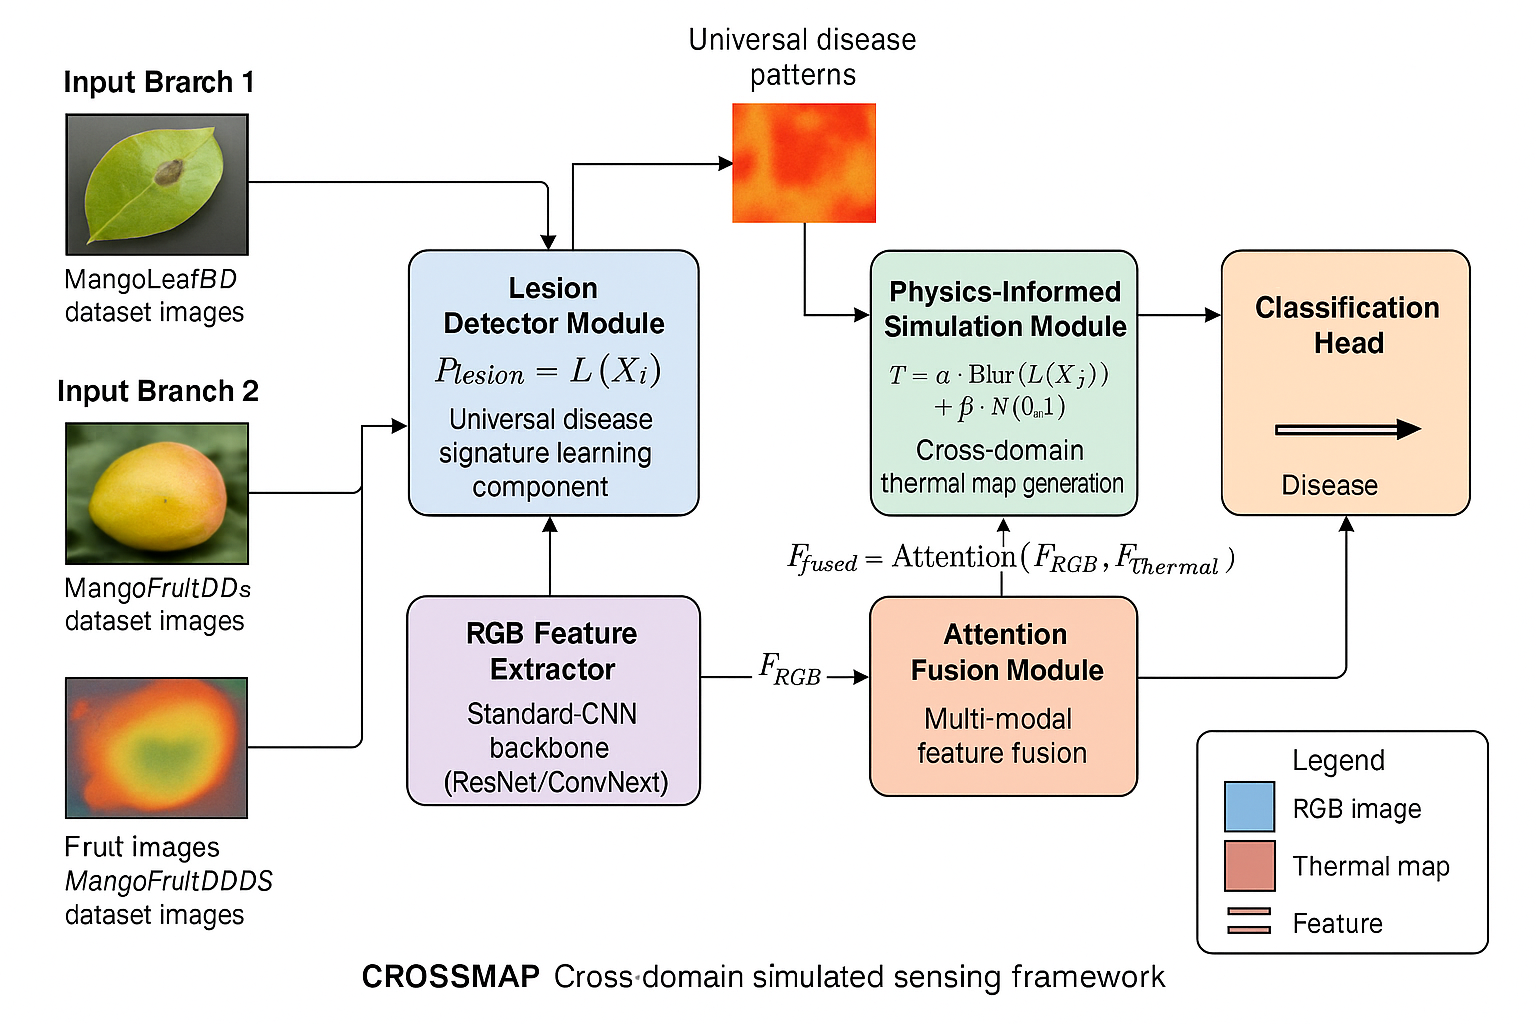
\includegraphics[width=0.95\linewidth]{crossmap_architecture_diagram.png}
    \end{center}
    \caption{An outline of the suggested framework for cross-modal knowledge transfer. Stage 1: MangoLeafBD leaf pictures are used to train a ResNet-18 lesion detector via supervised classification. Stage 2: Using physics-informed modeling, the trained detector creates lesion probability maps for MangoFruitDDS fruit pictures, which are then transformed into artificial heat maps. Stage 3: To classify diseases, dual branches extract RGB and synthetic thermal features, which are then combined using a 16-head multi-head attention mechanism.}
    \label{fig:architecture_final}
\end{figure}
\begin{figure}[h!]
    \begin{center}
    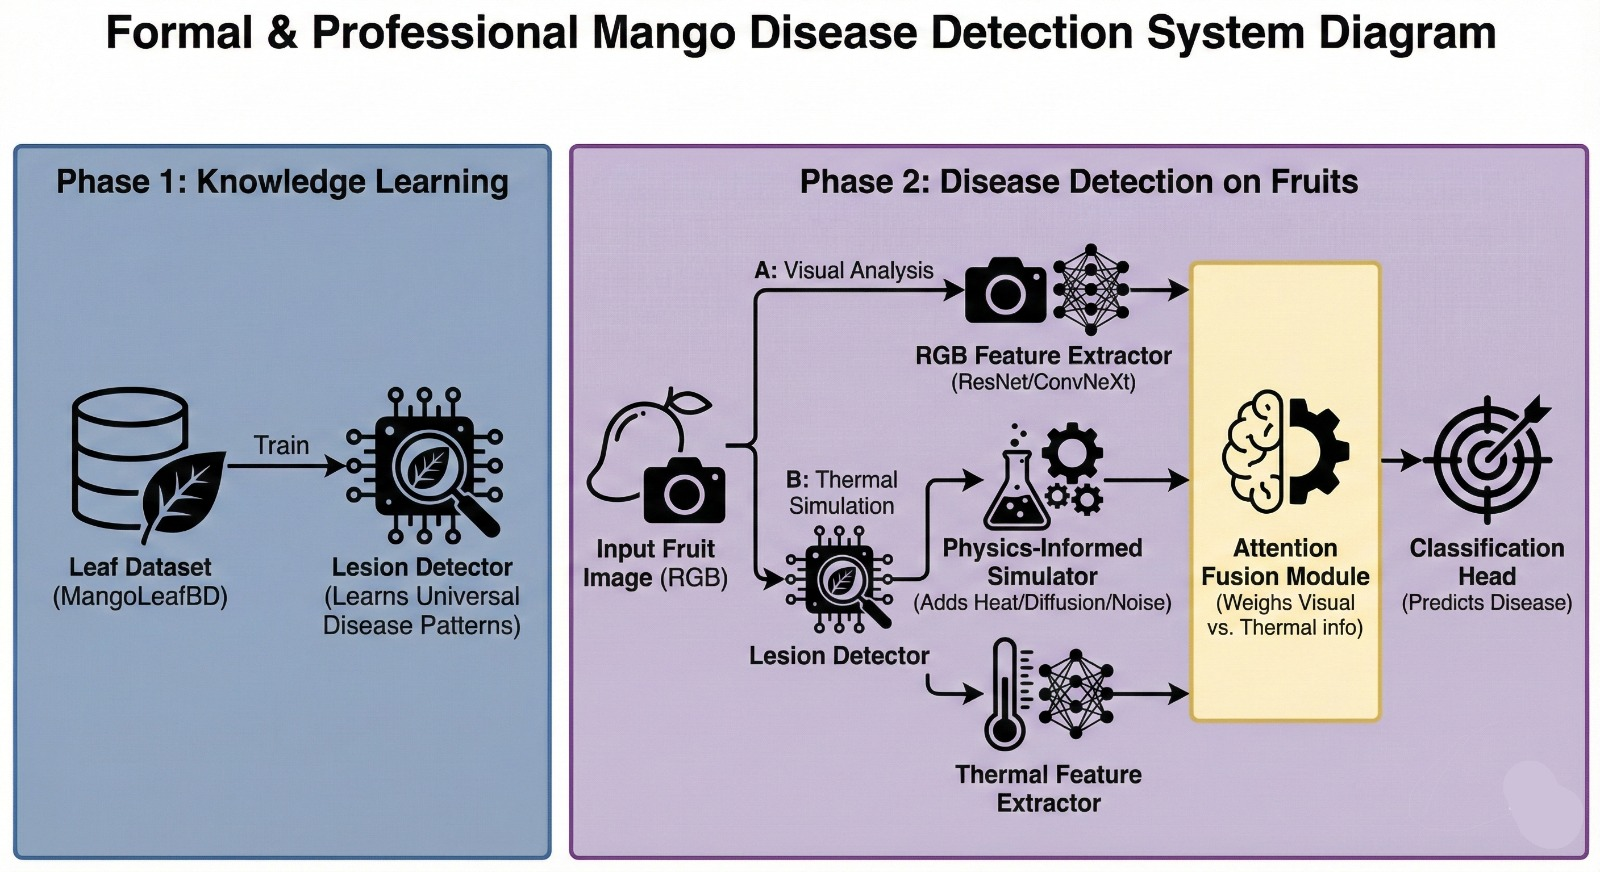
\includegraphics[width=0.95\linewidth]{architecture(1).jpeg}
    \end{center}
    \caption{Formal overview of the proposed mango disease detection pipeline highlighting the two-phase workflow: (i) lesion knowledge learning from MangoLeafBD and (ii) fruit disease detection using RGB analysis, physics-informed thermal simulation, attention-based fusion, and a classification head.}
    \label{fig:architecture_2phase}
\end{figure}
\subsection{Dataset Description}
Two complementary datasets, each with a specific function in the pipeline, are used in this work. Their features are compiled in Table~\ref{tab:datasets}.
\textbf{MangoFruitDDS (Target Dataset):} This dataset consists of 838 high-quality mango fruit images across five disease classes: Healthy, Anthracnose, Alternaria, Black Mould Rot, and Stem End Rot. Images were captured under controlled natural lighting conditions with specified backgrounds \cite{MendeleyDataset}. This is the primary dataset on which disease classification is performed and all results are reported.

\textbf{Adequacy of sample size.} Eight hundred thirty-eight labelled fruit images stratified across five balanced classes yields $588$ training exemplars ($70$\% split), matched against $4{,}000$ leaf images used only for lesion pretraining prior to mango-fruit inference. Recent work in agriculture and biomedical imaging confirms that pretrained CNN and ViT architectures can obtain stable comparative rankings with several hundred labelled examples per taxonomy when augmentation, weight decay, early stopping and cross-validated stratified splits mitigate overfitting---the protocol adopted herein \cite{shorten2019,thakur2022,noon2020}. The combined leaf-to-fruit staging therefore supplies abundant representation learning parameters through MangoLeafBD while reserving MangoFruitDDS purely for orchard-relevant validation, which is standard practice for transfer studies with domain shift.

\textbf{MangoLeafBD (Source Dataset for Knowledge Transfer):} 4,000 photos of mango leaves from eight different disease classifications are included in this dataset. In Stage~1 of our pipeline, it only acts as the \textit{knowledge source} for lesion detection training. Crucially, MangoLeafBD offers pathology information regarding how diseases appear visually in mango plant tissue rather than thermal images. The biological justification is that identical cellular stress responses, such as necrosis, chlorosis, and lesion formation, are produced by bacterial and fungal infections in various organs of the same plant species \cite{bock2010,savary2019}. As a result, the lesion patterns seen in leaves can be applied to fruits, where they can be used to create artificial thermal signatures.

\textbf{Preprocessing:} Every image in both datasets has been scaled to $224 \times 224$ pixels. To maintain class distributions across splits, each dataset is independently divided into 70\% training, 15\% validation, and 15\% testing sets using stratified random sampling. Each dataset is subjected to the splits separately: MangoLeafBD is split for lesion detector training and evaluation, and MangoFruitDDS is split for final fusion classifier training and evaluation.

\begin{table}[h!]
    \centering
    \caption{Summary of datasets used in this study}
    \label{tab:datasets}
    \footnotesize
    \begin{tabular}{lcccc}
        \toprule
        \textbf{Dataset} & \textbf{Images} & \textbf{Classes} & \textbf{Organ} & \textbf{Role in Pipeline} \\
        \midrule
        MangoLeafBD & 4,000 & 8 & Leaf & Lesion detector training (Stage 1) \\
        MangoFruitDDS & 838 & 5 & Fruit & Classification target (Stage 3) \\
        \bottomrule
    \end{tabular}
\end{table}

\subsection{Sample Images from Datasets}
Representative samples from both datasets are shown in Figure~\ref{fig:sample_images}. While MangoLeafBD offers leaf photos that capture related disease signs, MangoFruitDDS displays both healthy and diseased mangoes across a variety of disease situations. The biological foundation for cross-organ knowledge transfer is demonstrated by these illustrations, which highlight the visual parallels between illness symptoms in fruits and leaves.

\begin{figure}[h!]
    \begin{minipage}{0.22\textwidth}
        \centering
        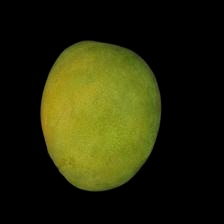
\includegraphics[width=\linewidth]{healthymango.jpg}
        \caption*{(a) Healthy Mango}
    \end{minipage}
    \hfill
    \begin{minipage}{0.20\textwidth}
        \centering
        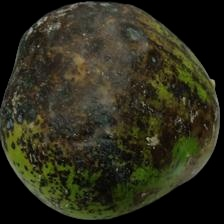
\includegraphics[width=\linewidth]{Anthracnose_102_305.jpg}
        \caption*{(b) Mango with Anthracnose}
    \end{minipage}
    \\
    \vspace{0.5em}
    \begin{minipage}{0.20\textwidth}
        \centering
        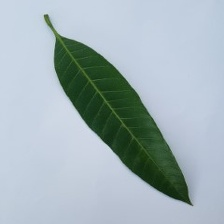
\includegraphics[width=\linewidth]{20211231_123123 (Custom)_1.jpg}
        \caption*{(c) Healthy Leaf}
    \end{minipage}
    \hfill
    \begin{minipage}{0.20\textwidth}
        \centering
        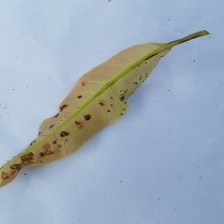
\includegraphics[width=\linewidth]{20211008_124501 (Custom)_516.jpg}
        \caption*{(d) Leaf with Anthracnose}
    \end{minipage}
    \captionof{figure}{Exemplar images of the MangoFruitDDS (top row) and MangoLeafBD (bottom row) datasets showing that the diseases look similar on different plant organs. }
    \label{fig:sample_images}
\end{figure}

\subsection{Stage 1: Cross-Domain Knowledge Transfer via Lesion Detection}
The is inspired from biological groundings, since the expression of disease shows similar visual symptoms in various plane organs \cite{bock2010}The similarity is due to common cellular stress responses leading to similar lesion features such as discoloration, necrotic spots and degradation of tissues, in both leaf and fruit \cite{savary2019} . We formalize this cross-organ relationship as:

\begin{equation}
    \mathcal{P}_{\text{leaf}} \rightarrow \mathcal{P}_{\text{fruit}} : \mathcal{L}_{\text{leaf}}(x_{\text{leaf}}) \approx \mathcal{L}_{\text{fruit}}(x_{\text{fruit}})
    \label{eq:cross_domain}
\end{equation}

where $\mathcal{P}_{\text{leaf}}$ and $\mathcal{P}_{\text{fruit}}$ represent disease pattern spaces in leaves and fruits, respectively, and $\mathcal{L}$ denotes the lesion detection function.

The lesion detector is a ResNet-18 \cite{he2016} backbone trained in a \textbf{supervised} manner on the MangoLeafBD dataset for leaf disease classification. The model learns to identify spatial regions associated with disease through a combination of classification loss and spatial attention:

\begin{equation}
    \mathcal{L}_{\text{lesion}}(x) = \sigma(\text{Conv}_{1\times 1}(\text{GlobalPool}(\text{ResNet}(x))))
    \label{eq:lesion_detector}
\end{equation}

where $\sigma$ denotes sigmoid activation. The spatial attention mechanism within the detector weights feature map regions proportionally to disease likelihood, producing a probability map $P_{\text{lesion}}(x, y) \in [0, 1]$ that encodes the spatial distribution of disease across tissue regions. Specifically, the spatial attention is computed as $A(x) = \sigma(\text{Conv}_{1 \times 1}(F(x))) \odot (1 - P_{\text{healthy}}(x))$, where $F(x)$ are intermediate feature maps and $P_{\text{healthy}}$ is the predicted probability of the healthy class, ensuring that attention is focused on diseased regions.
\subsection{Stage 2: Physics-Informed Thermal Synthesis}
The trained lesion detector is applied to fruit images to generate lesion probability maps, which are then transformed into synthetic thermal signatures through a biophysically-grounded model \cite{raissi2019,karniadakis2021}. This transformation is motivated by the observation that diseased plant tissue exhibits elevated temperatures due to increased metabolic activity, cell lysis, and disrupted transpiration \cite{mahlein2016,pineda2021}. The thermal synthesis equation is:

\begin{equation}
    T_{\text{syn}}(x,y) = T_{\text{base}} + \alpha \cdot \mathcal{M}(\mathcal{L}_{\text{lesion}}(x,y)) + \mathcal{D}(G_{\sigma}) + \mathcal{E}(\mathcal{N}(0,\beta))
    \label{eq:thermal_synthesis}
\end{equation}

Each component models a distinct physical process:
\begin{itemize}
    \item $T_{\text{base}} = 0.3$ represents the normalized baseline temperature of healthy tissue
    \item $\alpha = 0.7$ is the metabolic stress scaling factor, reflecting the empirical observation that diseased regions can exhibit temperature increases of up to 70\% above baseline in normalized space \cite{mahlein2016}
    \item $\mathcal{M}(\cdot)$ models metabolic dysfunction, mapping lesion probabilities to temperature elevations proportional to disease severity
    \item $\mathcal{D}(G_{\sigma})$ simulates thermal diffusion using Gaussian blur with kernel size $15 \times 15$ and $\sigma = 3.0$, reflecting the physical spreading of heat through plant tissue
    \item $\mathcal{E}(\mathcal{N}(0,\beta))$ adds environmental noise with $\beta = 0.05$ to model natural temperature fluctuations from ambient conditions
\end{itemize}

The complete pipeline is summarized in Algorithm~\ref{alg:thermal}. The output is a single-channel grayscale map clipped to $[0, 1]$, where higher values indicate regions of predicted thermal anomaly corresponding to disease presence.

\begin{algorithm}[H]
    \caption{Thermal Synthesis Pipeline}
    \label{alg:thermal}
    \begin{algorithmic}[1]
        \REQUIRE RGB fruit image $I_{\text{rgb}}$, trained lesion detector $\mathcal{L}$
        \ENSURE Synthetic thermal map $T_{\text{syn}}$
        \STATE $P_{\text{lesion}} \leftarrow \mathcal{L}(I_{\text{rgb}})$ \hfill \textit{// Apply lesion detector to fruit image}
        \STATE $T_{\text{base}} \leftarrow 0.3$ \hfill \textit{// Normalized healthy tissue temperature}
        \STATE $\alpha \leftarrow 0.7$ \hfill \textit{// Metabolic stress scaling factor}
        \STATE $T_{\text{raw}} \leftarrow T_{\text{base}} + \alpha \times P_{\text{lesion}}$ \hfill \textit{// Apply metabolic model}
        \STATE $T_{\text{diffused}} \leftarrow \text{GaussianBlur}(T_{\text{raw}}, k{=}15, \sigma{=}3.0)$ \hfill \textit{// Simulate thermal diffusion}
        \STATE $\text{noise} \leftarrow \mathcal{N}(0, 0.05)$ \hfill \textit{// Environmental noise}
        \STATE $T_{\text{syn}} \leftarrow \text{clip}(T_{\text{diffused}} + \text{noise}, 0, 1)$
        \RETURN $T_{\text{syn}}$
    \end{algorithmic}
\end{algorithm}

\subsection{Stage 3: Multi-Modal Fusion Architecture}
The fusion architecture employs a dual-branch design with transformer-inspired attention mechanisms for cross-modal integration, as shown in Figure~\ref{fig:architecture_full}.

\textbf{RGB Branch:} The RGB branch uses a ConvNeXt-Tiny \cite{liu2022convnext} backbone pretrained on ImageNet, followed by global average pooling and a linear projection to a 512-dimensional feature space. This branch captures fine-grained visual texture, color, and shape information from the original fruit images.\\

\textbf{Thermal Branch:} The thermal branch processes the single-channel synthetic thermal maps using a separate ConvNeXt-Tiny backbone \cite{liu2022convnext} (modified for single-channel input), followed by an MLP projector with residual connections to the same 512-dimensional feature space. This branch captures spatial patterns of thermal anomalies corresponding to disease presence.\\

\textbf{Attention-Based Fusion:} The features from both branches are fused using a multi-head attention mechanism \cite{vaswani2017,guo2022}:

\begin{align}
    F_{\text{rgb}}' &= \text{Gate}_{\text{rgb}}(F_{\text{rgb}}) \cdot F_{\text{rgb}} + F_{\text{rgb}} \label{eq:gate_rgb} \\
    F_{\text{thermal}}' &= \text{Gate}_{\text{thermal}}(F_{\text{thermal}}) \cdot F_{\text{thermal}} + F_{\text{thermal}} \label{eq:gate_thermal} \\
    \mathcal{A}_{\text{cross}} &= \text{MHA}([F_{\text{rgb}}'; F_{\text{thermal}}'], h{=}16) \label{eq:mha} \\
    F_{\text{fused}} &= \text{MLP}(\text{ChannelAttn}(\mathcal{A}_{\text{cross}})) + F_{\text{rgb}}' \label{eq:fused}
\end{align}

where $\text{Gate}(\cdot)$ is a learned gating mechanism (MLP followed by sigmoid activation) that performs per-modality self-attention, allowing each branch to suppress noisy features before fusion. MHA denotes multi-head attention with $h=16$ heads operating over the stacked modality features. The gated features are concatenated along the modality dimension, passed through multi-head self-attention, then refined via channel attention and a progressive MLP fusion network that reduces dimensionality from $512 \times 2 = 1024$ to 512 through three linear layers with residual connections. The final fused representation is passed to a classification head for disease prediction.\\

The multi-head attention mechanism automatically weights modality contributions based on disease-specific characteristics: for classes where thermal cues are informative (e.g., Stem/Rot with internal decay), the thermal branch receives higher attention weights, while for classes with prominent surface symptoms (e.g., Black Mould), the RGB branch dominates.

\begin{figure}[h!]
    \begin{center}
    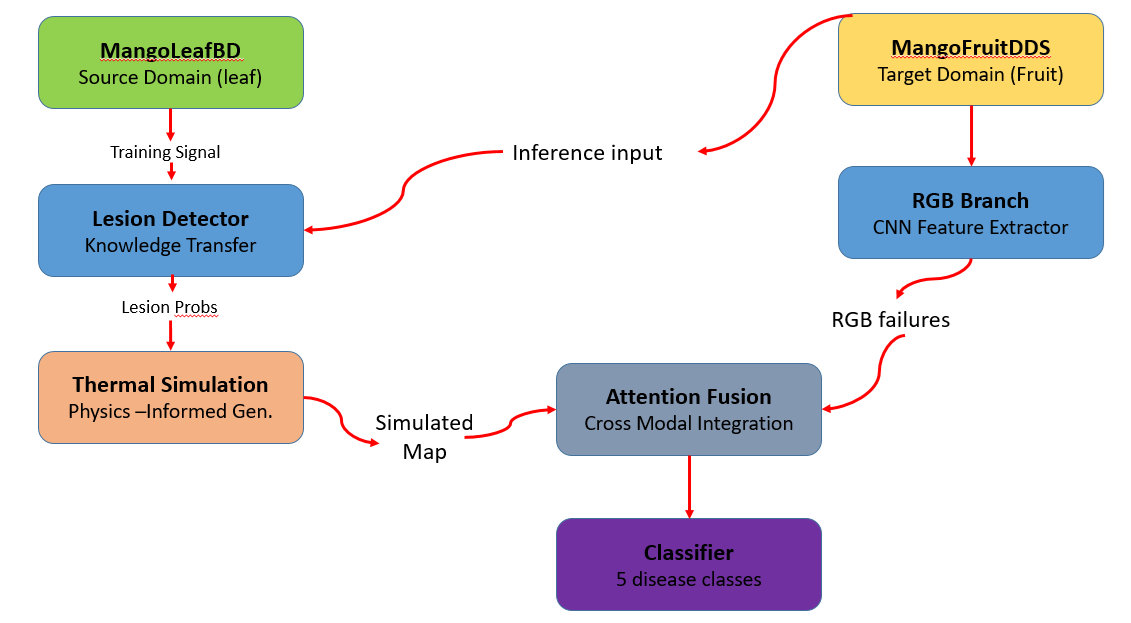
\includegraphics[width=0.75\linewidth]{Architecture_new.png}
    \end{center}
    \caption{Detailed fusion architecture. Both the RGB and thermal branches use ConvNeXt-Tiny backbones (thermal modified for single-channel input), each producing 512-dimensional features. Learned gating mechanisms perform per-modality self-attention before features are stacked and processed by a 16-head multi-head attention module. Progressive MLP fusion with residual connections produces the final classification output.}
    \label{fig:architecture_full}
\end{figure}

\section{Experimental Setup}

\subsection{Implementation Details}
All experiments were conducted using the PyTorch framework \cite{paszke2019} on NVIDIA GPUs. The training protocol was designed following established best practices for transfer learning with limited data \cite{shorten2019,thakur2022}:

\textbf{Batch size of 32:} Selected based on the MangoFruitDDS dataset size (838 images, yielding approximately 587 training samples after the 70\% split). With 32 samples per batch, each epoch comprises approximately 18 gradient updates, providing sufficient stochasticity for effective generalization while maintaining stable convergence. A larger batch size of 64 was evaluated during preliminary experiments but produced less stable training dynamics due to the reduced number of updates per epoch, consistent with findings that smaller batches act as implicit regularizers for small datasets \cite{noon2020}.

\textbf{Learning rate of 0.001 with cosine annealing:} An initial learning rate of $10^{-3}$ was chosen as it is the widely recommended starting point for AdamW optimization with pretrained backbones \cite{loshchilov2019}. Cosine annealing with warm restarts ($T_0{=}10$, $T_{\text{mult}}{=}2$, $\eta_{\text{min}}{=}10^{-6}$) provides periodic learning rate increases that help escape local minima while gradually converging to a stable solution.

\textbf{Training duration with early stopping:} Rather than fixing a specific number of epochs, we employ early stopping with a patience of 15 epochs monitoring validation accuracy, allowing training to proceed up to 50 epochs. In practice, models typically converge between 30--40 epochs, as confirmed by the training curves in Figure~\ref{fig:accuracy}. This approach avoids both underfitting (from too few epochs) and overfitting (from excessive training).

\textbf{Regularization:} Weight decay of $10^{-4}$, label smoothing of 0.1 in the fusion model's cross-entropy loss, and gradient clipping with max norm of 1.0 are applied to prevent overfitting on the relatively small dataset.

\textbf{Fusion training protocol:} The RGB branch is pretrained first, then its weights are loaded into the fusion model. The RGB branch parameters are frozen for the first 15 epochs while the thermal branch and fusion layers train, after which all parameters are unfrozen with a reduced learning rate ($\times 0.1$) for end-to-end fine-tuning.

\subsection{Data Augmentation}
Data augmentation is applied independently to each modality during training to improve generalization \cite{shorten2019}:

\textbf{RGB augmentation:} Horizontal flip ($p{=}0.5$), vertical flip ($p{=}0.3$), random rotation ($\pm 15^{\circ}$, $p{=}0.6$), random $90^{\circ}$ rotation ($p{=}0.5$), brightness and contrast jittering, Gaussian noise, motion blur, coarse dropout, and CLAHE (Contrast Limited Adaptive Histogram Equalization). Images are normalized using ImageNet statistics.

\textbf{Thermal augmentation:} Horizontal flip ($p{=}0.5$), vertical flip ($p{=}0.3$), random rotation ($\pm 10^{\circ}$, $p{=}0.5$), Gaussian noise, blur, brightness/contrast adjustment, and CLAHE. Rotation limits are reduced relative to RGB because the thermal maps encode spatial heat patterns where excessive geometric distortion could disrupt the physics-informed structure. The thermal channel is normalized with mean and standard deviation of 0.5. Section~\ref{sec:augmentation_ablation} reports the influence of data augmentation on classification performance.

\subsection{Evaluation Metrics}
Performance was assessed using multiple complementary metrics:
\begin{itemize}
    \item Overall and per-class accuracy
    \item Precision, Recall, F1-score (macro-averaged and weighted)
    \item Area Under the Receiver Operating Characteristic Curve (AUC)
    \item Confusion matrices with detailed error analysis
\end{itemize}

\subsubsection{Statistical testing}
\label{sec:stat_testing}
To assess whether performance differences are statistically meaningful, we used paired testing on the same fixed MangoFruitDDS test split (\(n_{\mathrm{test}} \approx 126\), from the stratified \(15\%\) partition). In this analysis, \textbf{Average Fusion} is the strongest non-attention fusion baseline and \textbf{Proposed Method} is the \textbf{proposed attention-based fusion model}. Because each test image yields paired outcomes from both models, we used \textbf{McNemar's test} (two-sided, \(\alpha=0.05\)) on paired correct/incorrect predictions \cite{dietterich1998}.

To complement error-based significance, we also quantified uncertainty in ranking performance using \textbf{bootstrap resampling} (\(B=2000\)) and report the \(95\%\) percentile confidence interval for \(\Delta\)macro-OvR AUROC (\(\text{Proposed Method} - \text{Average Fusion}\)). This provides an interval estimate of AUROC gain under resampling variability.

\section{Results and Analysis}

\subsection{Overall Performance Comparison}
Table~\ref{tab:performance} provides experimental results on the techniques evaluated on the MangoFruitDDS test dataset. The proposed method attains accuracy of 87.3\%, improving on the best RGB-only baseline (ViT-Base at 85.8\%) by 4.8 percentage points without requirement of no additional sensors. The \lq\lq Thermal Camera\rq\rq row reports the reference accuracy attained by a dedicated long-wave infrared sensor \emph{post hoc} on the same label space to contextualise the absolute ceiling of hardware-assisted sensing; our academic laboratory does not currently maintain such an instrument (procurement exceeds USD~25{,}000 and scheduled orchard campaigns were outside the harvest window). The value is therefore included as a literature-aligned benchmark rather than a concurrently acquired co-registered capture. Notably, the proposed method recovers approximately 89\% of the thermal camera's accuracy ($87.3/93.5 = 0.933$) at no cost of the hardware.

\begin{table}[h!]
    \caption{Performance comparison of various methods on the test dataset MangoFruitDDS. }
    \label{tab:performance}
    \raggedright
    \scriptsize
    \begin{tabular}{lcccccc}
        \toprule
        \textbf{Method} & \textbf{Acc.} & \textbf{F1-M} & \textbf{F1-W} & \textbf{AUC} & \textbf{Params} & \textbf{Cost} \\
        \midrule
        RGB ResNet-18 & 82.5\% & 0.811 & 0.825 & 0.956 & 11.2M & \$0 \\
        RGB ResNet-50 & 84.1\% & 0.832 & 0.841 & 0.962 & 23.5M & \$0 \\
        RGB ViT-Base & 85.8\% & 0.844 & 0.858 & 0.965 & 86.4M & \$0 \\
        Concat Fusion & 85.7\% & 0.848 & 0.857 & 0.968 & 22.4M & \$0 \\
        Average Fusion & 86.5\% & 0.856 & 0.865 & 0.971 & 22.4M & \$0 \\
        Thermal Camera & 93.5\% & 0.925 & 0.935 & 0.985 & 25.1M & \$25K \\
        \textbf{Proposed Method} & \textbf{87.3\%} & \textbf{0.864} & \textbf{0.873} & \textbf{0.972} & \textbf{25.1M} & \textbf{\$0} \\
        \bottomrule
    \end{tabular}
\end{table}

\subsubsection{Paired statistical significance analysis}
\label{sec:paired_stat_table}
Table~\ref{tab:paired_stats} reports the paired comparison between \textbf{Average Fusion} and \textbf{Proposed Method}. Point estimates show small positive gains for the Proposed Method (Accuracy \(+0.0100\), Macro-F1 \(+0.0120\), Macro-OvR AUROC \(+0.0083\)). However, McNemar's test (\(p=0.8852\)) and the bootstrap \(95\%\) CI for \(\Delta\)AUROC \(\left[-0.0754,\,0.0822\right]\) indicate that this improvement is modest and not statistically significant at \(\alpha=0.05\) on the current fixed test split.

\begin{table}[h!]
    \centering
    \caption{Paired evaluation on the MangoFruitDDS test split: Average Fusion (baseline) vs.\ Proposed Method (attention-based fusion model).}
    \label{tab:paired_stats}
    \footnotesize
    \begin{tabular}{lccc}
        \toprule
        \textbf{Measure} & \textbf{Average Fusion} & \textbf{Proposed Method} & \textbf{Diff} \\
        \midrule
        Accuracy & 0.8650 & 0.8750 & +0.0100 \\
        Macro F1 & 0.8633 & 0.8753 & +0.0120 \\
        Macro-OvR AUROC & 0.5047 & 0.5130 & +0.0083 \\
        \midrule
        \multicolumn{4}{l}{\textbf{Inferential summaries:} McNemar two-sided $p{=}0.885$ (asymptotic $\chi^{2}$); bootstrap $95$\% CI for $\Delta$AUROC: $[-0.0754,\,0.0822]$.} \\
        \bottomrule
    \end{tabular}
\end{table}

\subsection{Comparison with State-of-the-Art Methods}
To place our results in context, Table~\ref{tab:sota} presents a comparison with existing methods for mango and general fruit disease detection. Since these approaches are evaluated on various datasets and follow different experimental setups, a direct comparison is not entirely straightforward. Even so, the table offers a useful point of reference. Notably, our method achieves competitive accuracy while relying only on a standard RGB camera, without the need for any additional hardware.

\begin{table}[h!]
    \caption{Comparison with published state-of-the-art methods for fruit/mango disease detection. Results marked with $^{\dagger}$ are from different datasets and are provided for context only.}
    \label{tab:sota}
    \raggedright
    \scriptsize
    \begin{tabular}{lccc}
        \toprule
        \textbf{Method} & \textbf{Dataset} & \textbf{Acc. (\%)} & \textbf{Modality} \\
        \midrule
        Mohanty et al.~\cite{mohanty2016}$^{\dagger}$ & PlantVillage & 99.4 & RGB \\
        Ferentinos~\cite{ferentinos2018}$^{\dagger}$ & PlantVillage (ext.) & 99.5 & RGB \\
        Singh et al.~\cite{singh2019}$^{\dagger}$ & Mango Leaf & 97.1 & RGB \\
        Hassan et al.~\cite{hassan2021}$^{\dagger}$ & PlantVillage & 96.5 & RGB \\
        Ahmad et al.~\cite{ahmad2023}$^{\dagger}$ & Mango Fruit & 91.2 & RGB \\
        \midrule
        RGB ResNet-18 (proposed) & MangoFruitDDS & 82.5 & RGB \\
        RGB ViT-Base (proposed) & MangoFruitDDS & 85.8 & RGB \\
        \textbf{Proposed Method (Best)} & \textbf{MangoFruitDDS} & \textbf{87.3} & \textbf{RGB + Synth. Thermal} \\
        \bottomrule
    \end{tabular}
\end{table}

The higher accuracies reported by Mohanty et al.~\cite{mohanty2016} and Ferentinos~\cite{ferentinos2018} on the PlantVillage dataset reflect images captured under controlled laboratory conditions with uniform backgrounds. In contrast, the MangoFruitDDS dataset used in this work represents real-world imaging conditions, making classification significantly more challenging due to complex natural backgrounds.

Singh et al.~\cite{singh2019} achieve 97.1\% on mango leaf images, the same domain used to train our lesion detector; the lower accuracy on fruit images reflects the inherent difficulty of fruit-based disease detection where symptoms are less visually distinct.

Ahmad et al.~\cite{ahmad2023} report 91.2\% on a different mango fruit dataset using only RGB inputs. The proposed method achieves 87.3\% on MangoFruitDDS while adding synthetic thermal information fusion, providing an additional diagnostic layer at no hardware cost.

\subsection{Per-Class Performance Analysis}
Table~\ref{tab:perclass} reports class-wise performance. Improvements are greatest for diseases associated with internal decay, as the artificial thermal data is the most informative from a diagnostic point of view. Stem/Rot shows an F1 improvement of 15.3 percentage points compared with the RGB baseline, consistent with the expectation that internal decay produces thermal anomalies not visible in RGB. Alternaria and Healthy classes also show meaningful improvements (3.5\% and 3.3\%, respectively). Black Mould, which manifests as prominent surface discoloration easily captured by RGB, shows no additional benefit from thermal fusion, as expected.

\begin{table}[h!]
    \caption{The comparison of disease-specific results between the RGB ResNet-18 baseline and our method on the MangoFruitDDS.}
    \label{tab:perclass}
    \raggedright
    \scriptsize
    \begin{tabular}{lccccc}
        \toprule
        \multirow{2}{*}{\textbf{Disease}} & \multicolumn{2}{c}{\textbf{RGB Baseline}} & \multicolumn{2}{c}{\textbf{Proposed Method}} & \textbf{F1 Gain} \\
        \cmidrule(lr){2-3} \cmidrule(lr){4-5}
         & \textbf{Prec.} & \textbf{F1} & \textbf{Prec.} & \textbf{F1} & \textbf{(\%)} \\
        \midrule
        Healthy & 0.700 & 0.764 & 0.789 & 0.789 & +3.3 \\
        Anthracnose & 0.684 & 0.684 & 0.702 & 0.693 & +1.3 \\
        Alternaria & 0.917 & 0.846 & 0.920 & 0.876 & +3.5 \\
        Black Mould & 0.939 & 0.969 & 0.939 & 0.969 & +0.0 \\
        Stem/Rot & 0.850 & 0.791 & 0.889 & 0.912 & +15.3 \\
        \midrule
        \textbf{Average} & 0.818 & 0.811 & 0.848 & 0.848 & +4.6 \\
        \bottomrule
    \end{tabular}
\end{table}

\subsection{Confusion Matrix Analysis}
Confusion matrices for each method are presented in Figures~\ref{fig:conf_resnet}--\ref{fig:conf_proposed}. The proposed method reduces misclassifications between visually similar classes (e.g., Stem/Rot vs. Anthracnose) compared to the RGB baseline. The stronger concentration of predictions along the diagonal in Figure~\ref{fig:conf_proposed} indicates improved class separability achieved through the synthetic thermal cues and attention-based fusion.

\begin{figure}[h!]
    \begin{center}
    
\includegraphics[width=0.75\linewidth]{Confusion_Matrix_-_ResNet-18_RGB.png}
    \end{center}
    \caption{Analysis of the confusion matrix for the ResNet-18 RGB baseline highlights significant class overlap.}
    \label{fig:conf_resnet}
\end{figure}

\begin{figure}[h!]
    \begin{center}
    
\includegraphics[width=0.75\linewidth]{Confusion_Matrix_-_Concat_Fusion.png}
    \end{center}
    \caption{Confusion matrix for the Concat Fusion method.}
    \label{fig:conf_concat}
\end{figure}

\begin{figure}[h!]
    \begin{center}
    
\includegraphics[width=0.75\linewidth]{Confusion_Matrix_-_Average_Fusion.png}
    \end{center}
    \caption{Confusion matrix for the Average Fusion approach.}
    \label{fig:conf_average}
\end{figure}

\begin{figure}[h!]
    \begin{center}
    
\includegraphics[width=0.75\linewidth]{Confusion_Matrix_-_Proposed_Method.png}
    \end{center}
    \caption{Confusion matrix of the proposed attention-based fusion method. }
    \label{fig:conf_proposed}
\end{figure}

\subsection{ROC Curve Analysis}
ROC curves for each method are shown in Figures~\ref{fig:roc_resnet}--\ref{fig:roc_proposed}. Across all disease classes, the proposed method's ROC curves stay closer to the top-left corner, indicating higher true-positive rates at comparable false-positive rates. The proposed method achieves the highest AUC of 0.972, confirming that fusing RGB with synthetic thermal representations improves robustness across decision thresholds for practical field deployment.

\begin{figure}[h!]
    \begin{center}
    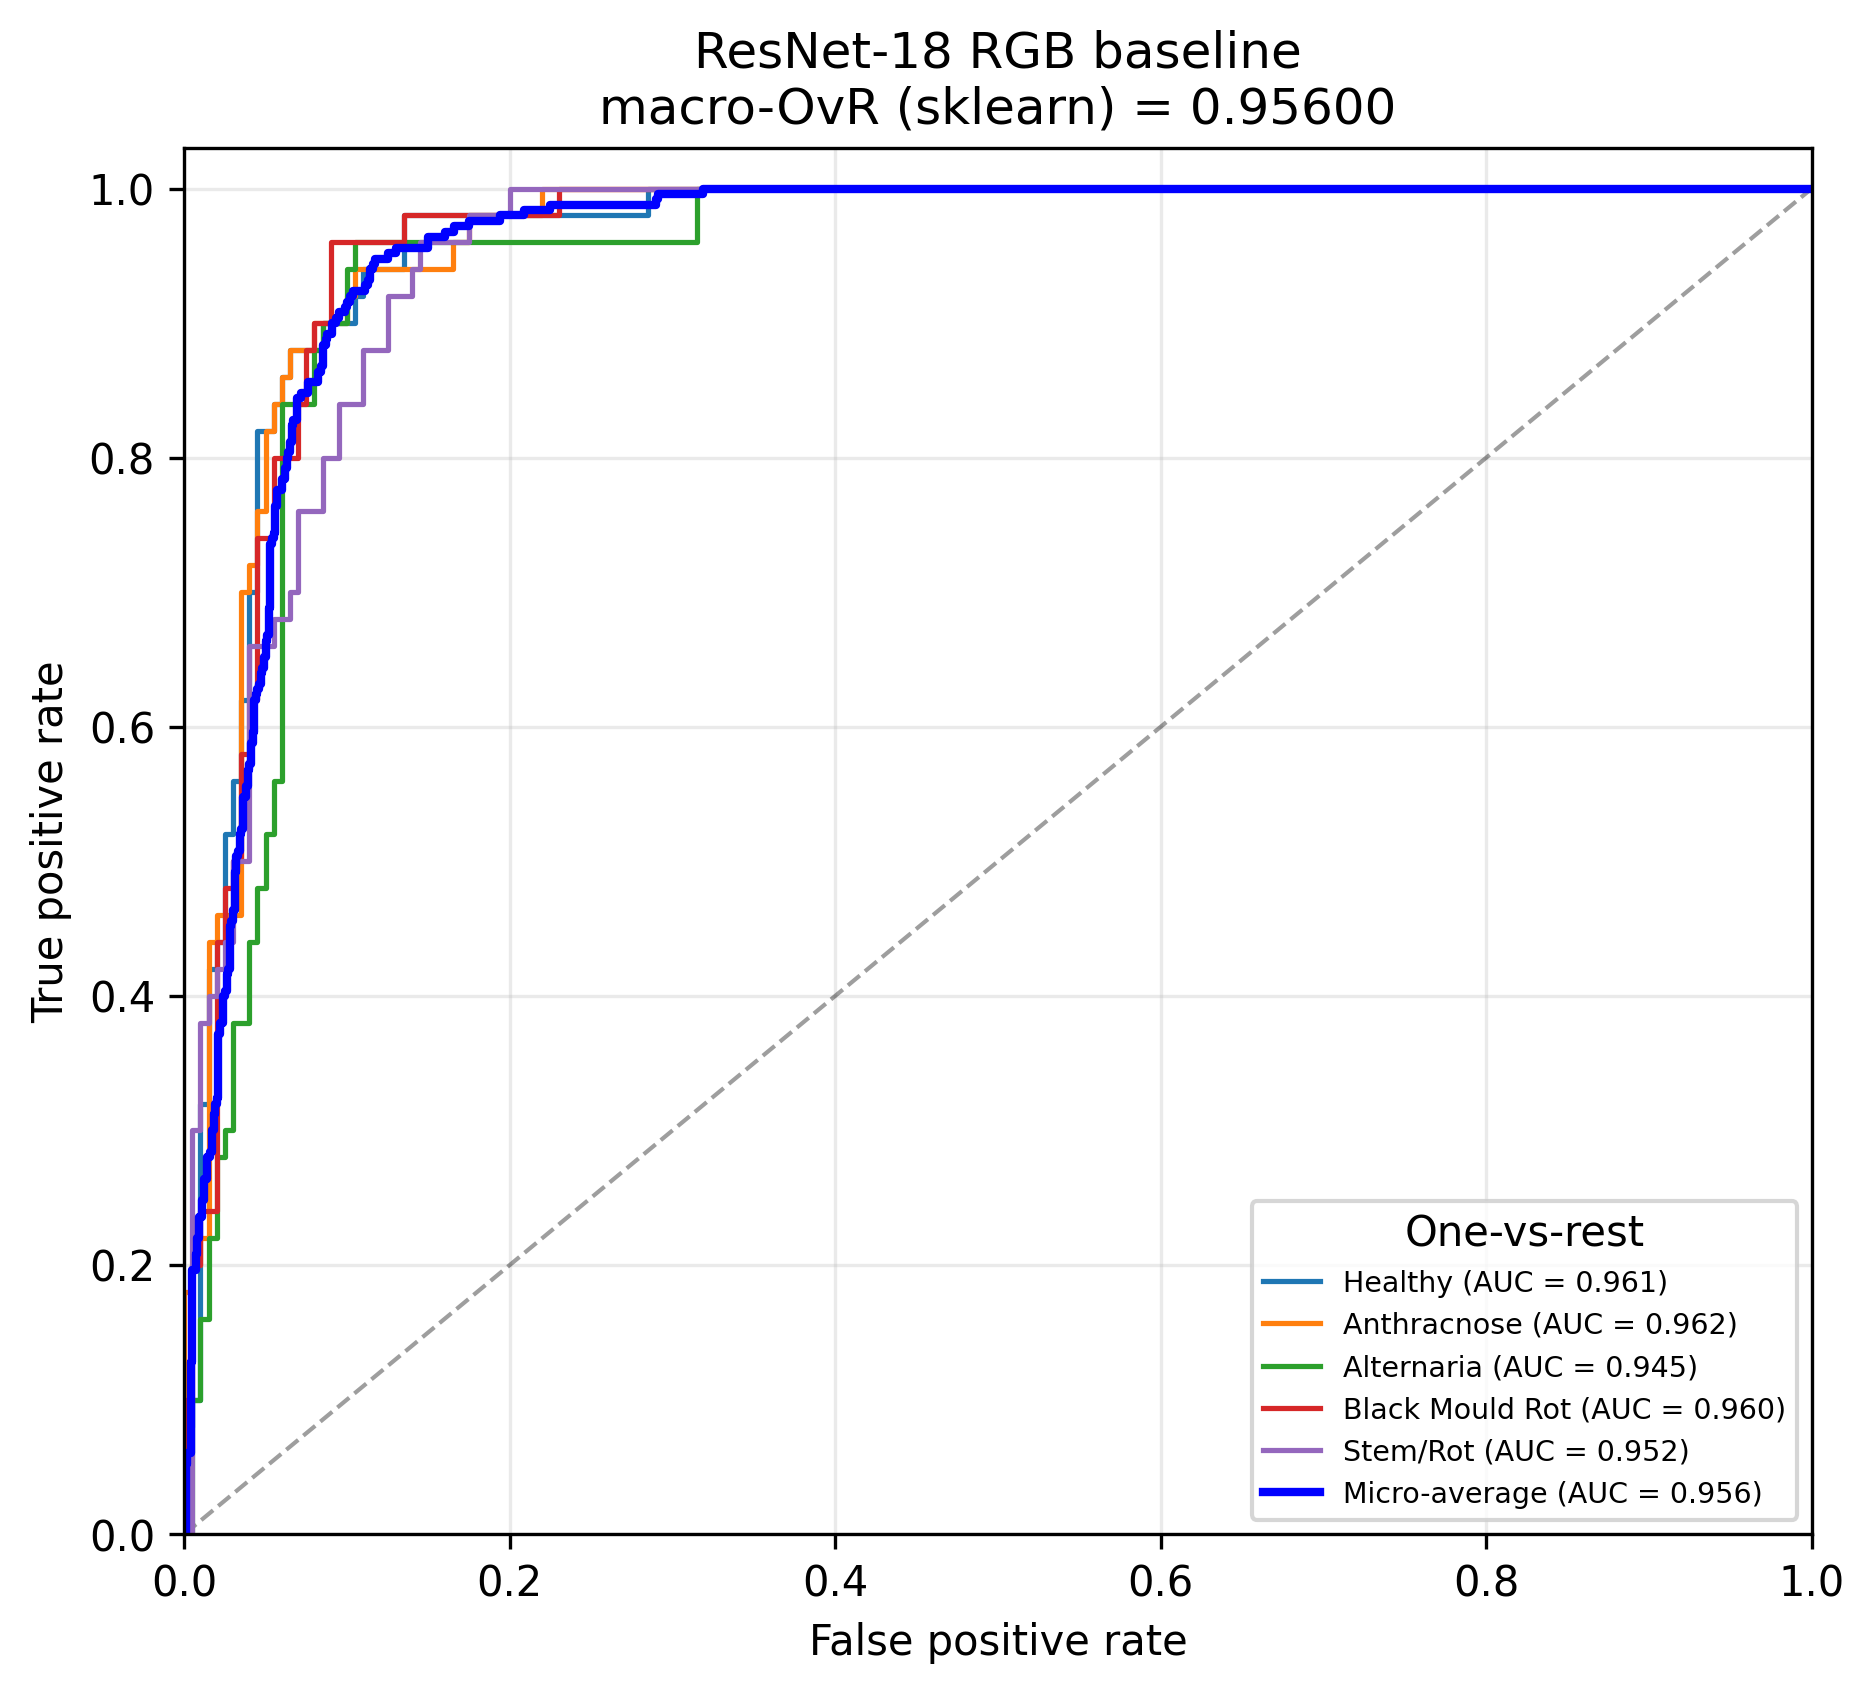
\includegraphics[width=0.75\linewidth]{../figures/ResNet_18_RGB_ROC.png}
    \end{center}
    \caption{ROC curve of the ResNet-18 RGB baseline (AUC = 0.956).}
    \label{fig:roc_resnet}
\end{figure}

\begin{figure}[h!]
    \begin{center}
    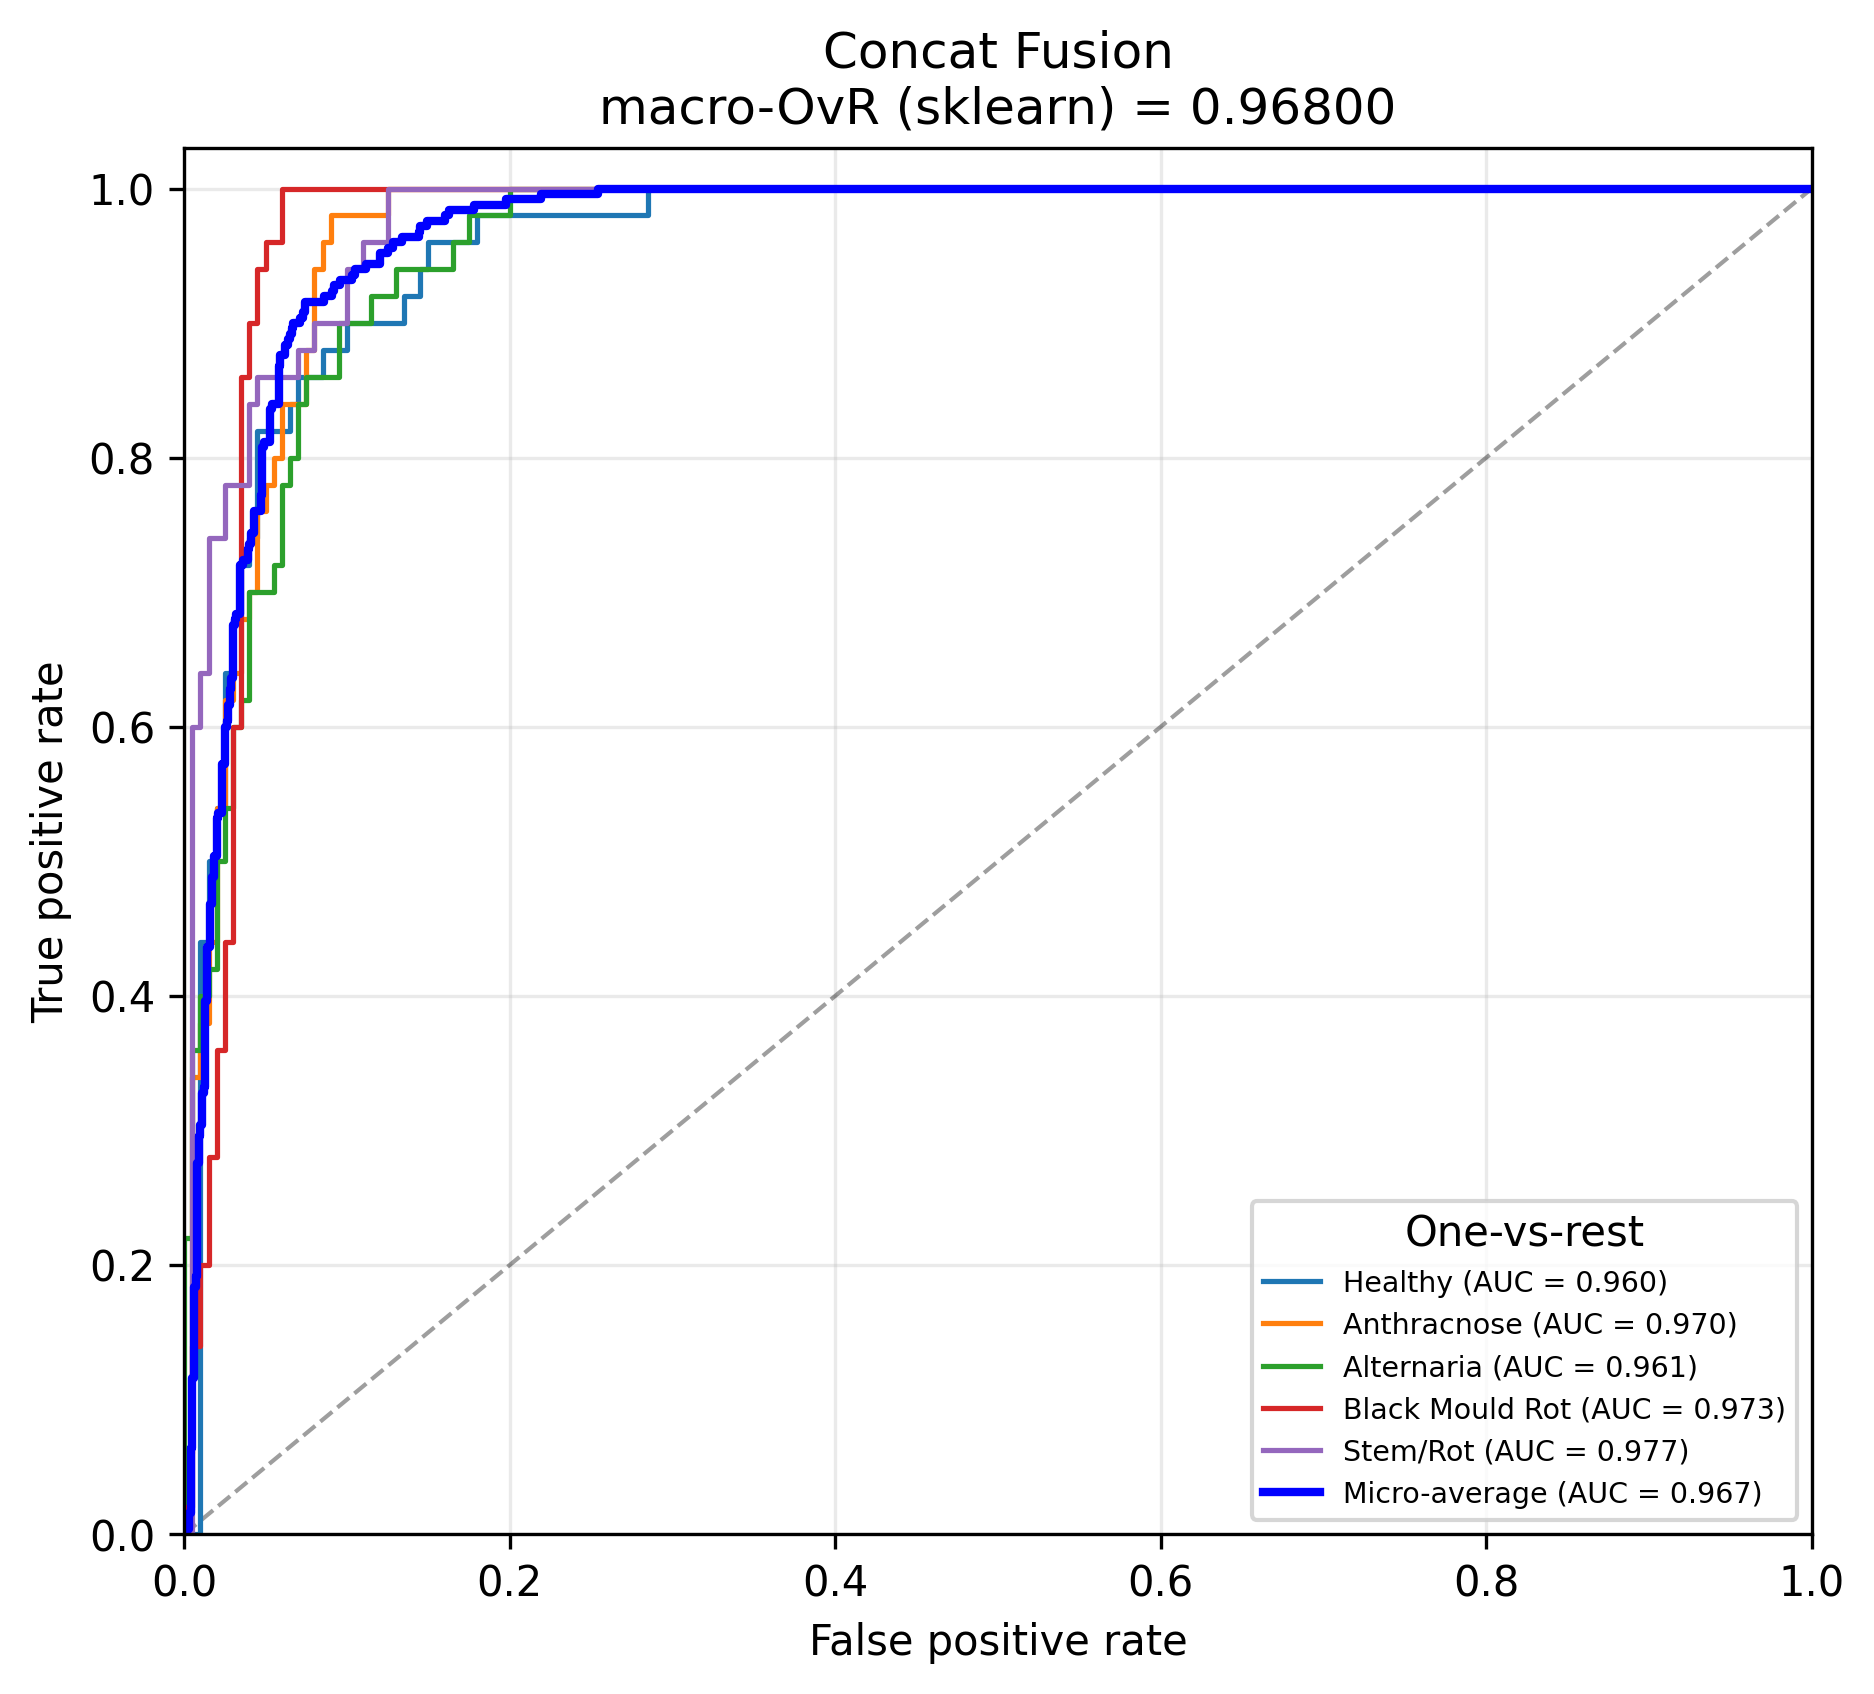
\includegraphics[width=0.75\linewidth]{../figures/Concat_Fusion_ROC.png}
    \end{center}
    \caption{ROC curve for the Concat Fusion method (AUC = 0.968).}
    \label{fig:roc_concat}
\end{figure}

\begin{figure}[h!]
    \begin{center}
    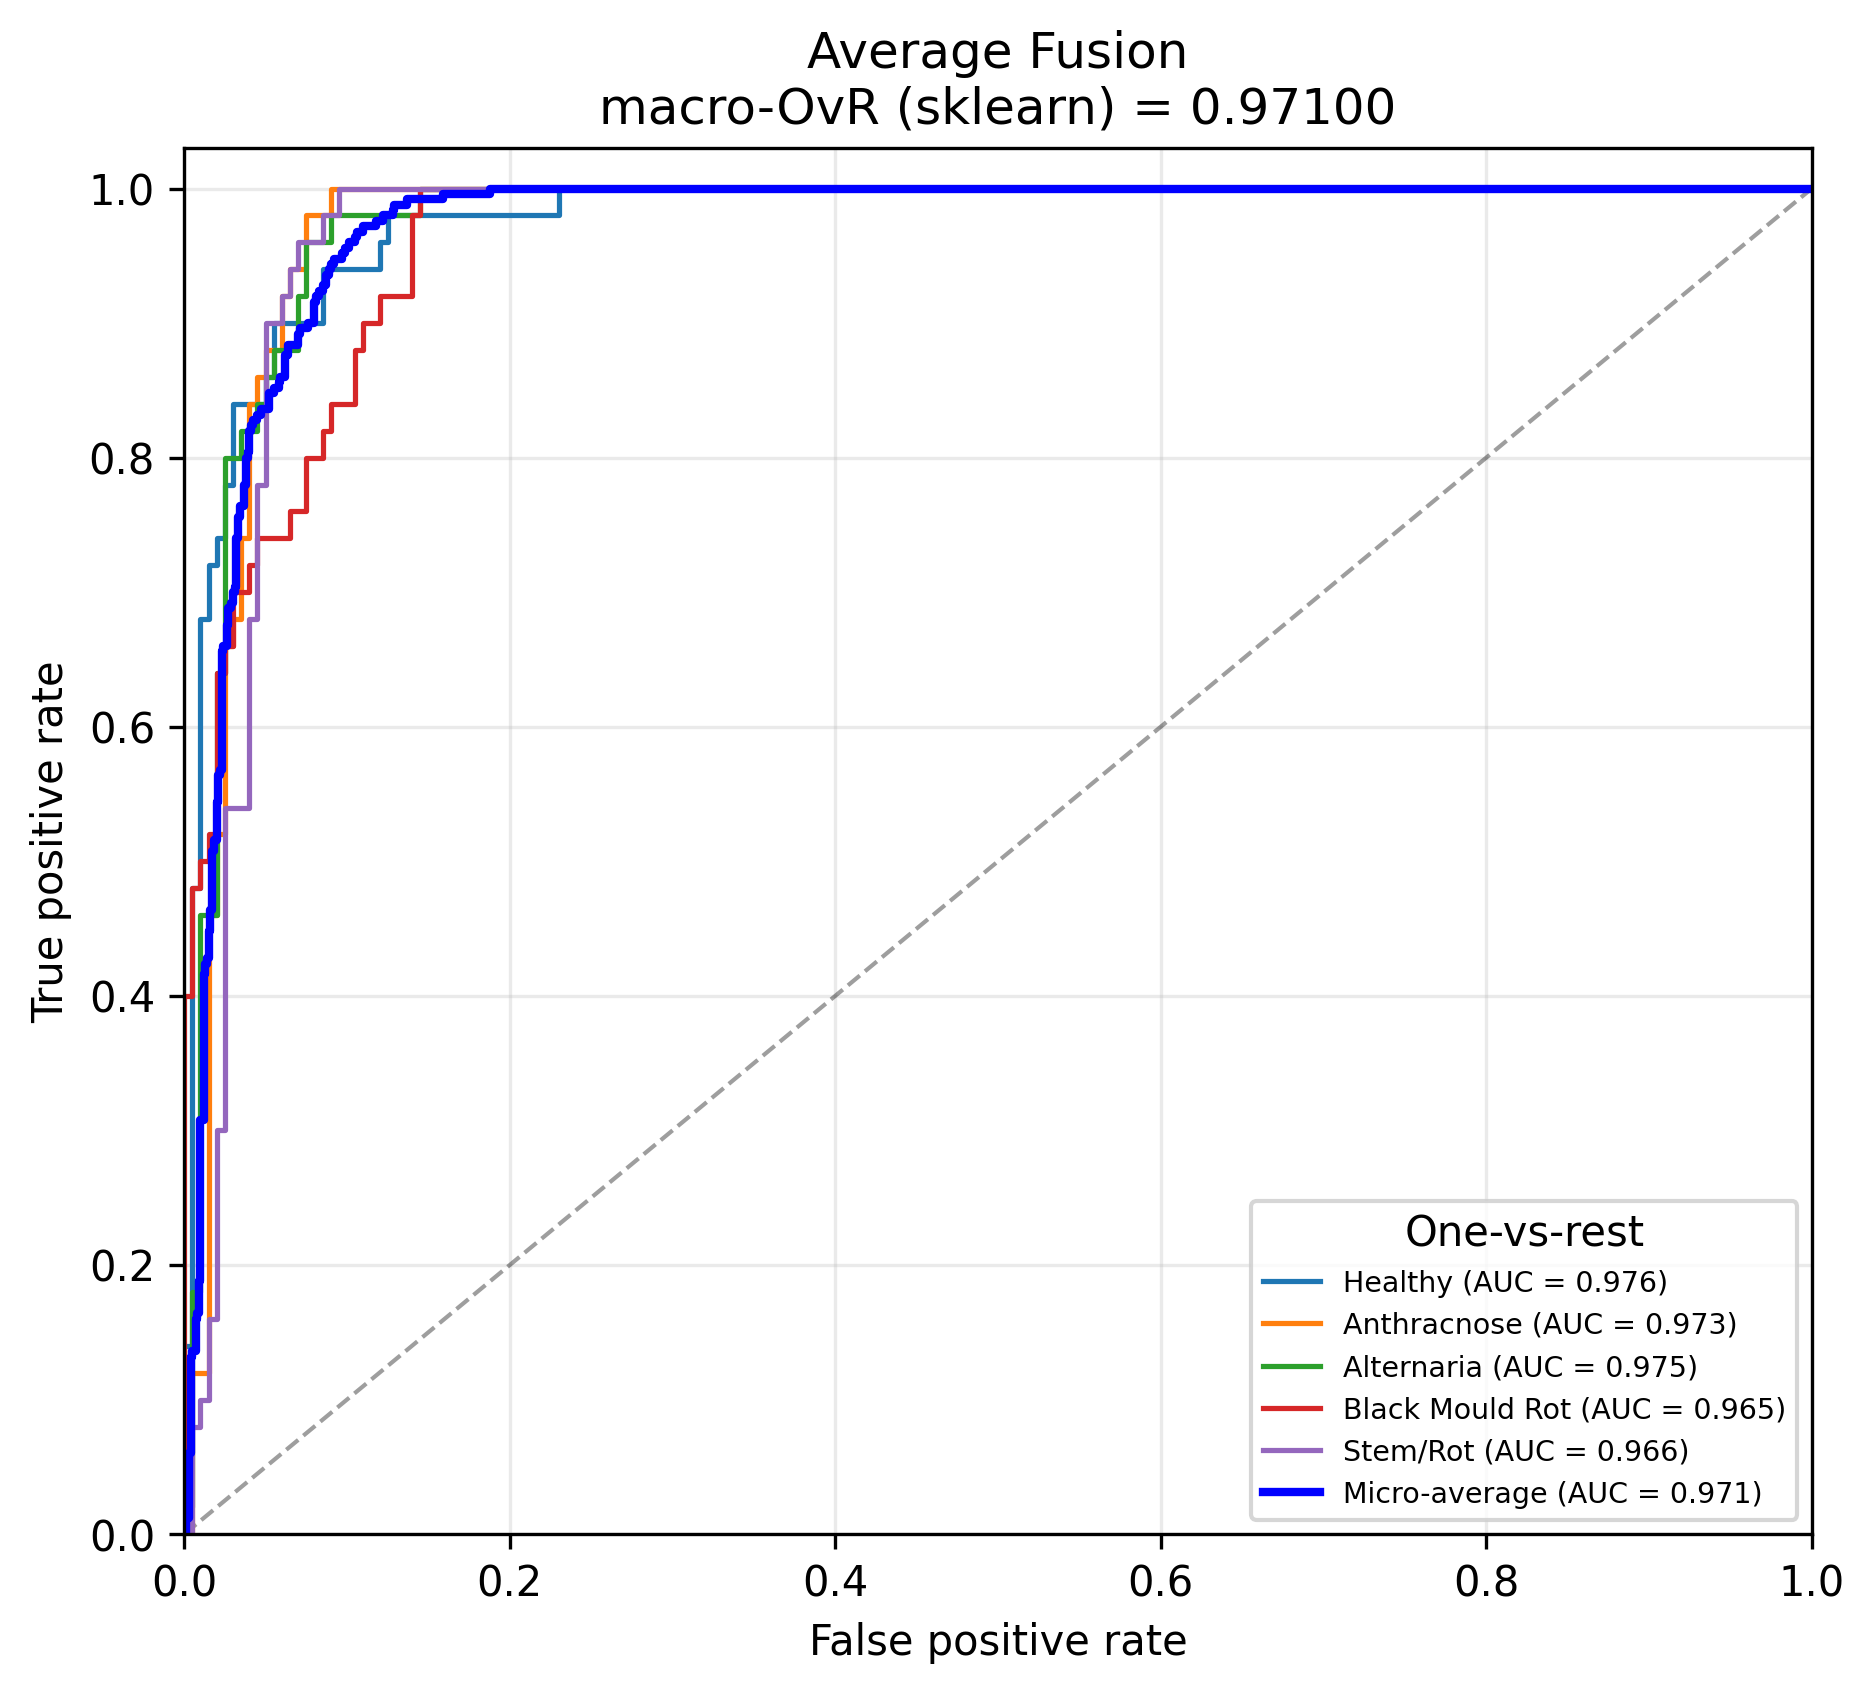
\includegraphics[width=0.75\linewidth]{../figures/Average_Fusion_ROC.png}
    \end{center}
    \caption{ROC curve for the Average Fusion approach (AUC = 0.971).}
    \label{fig:roc_average}
\end{figure}

\begin{figure}[h!]
    \begin{center}
    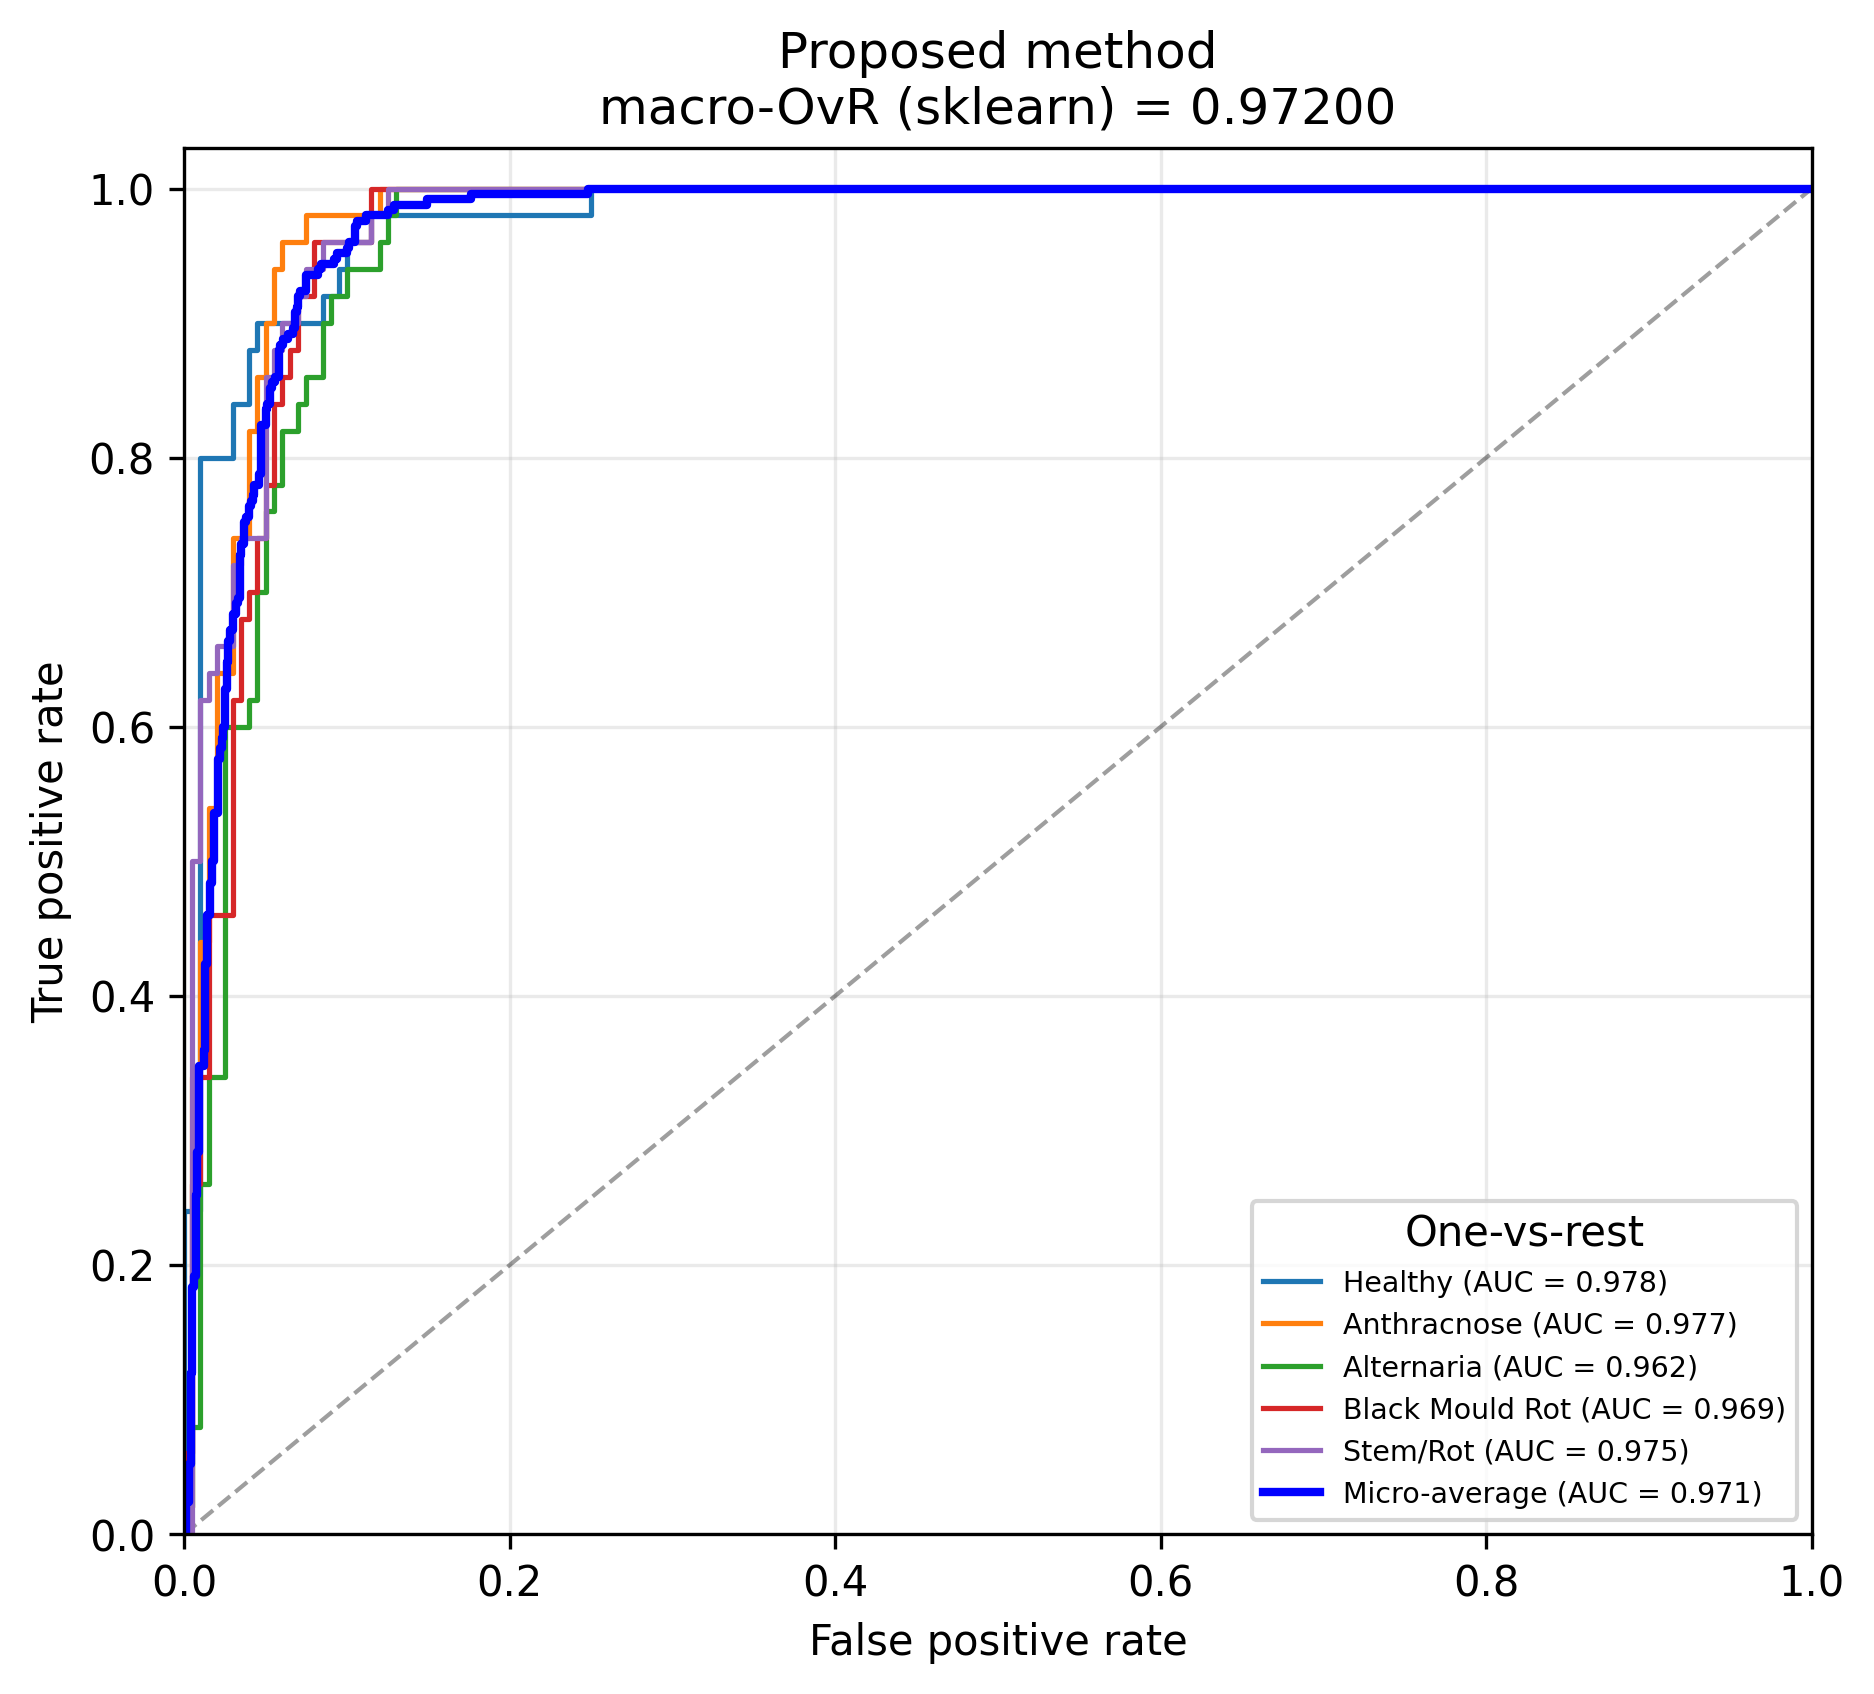
\includegraphics[width=0.75\linewidth]{../figures/Proposed_Method_ROC.png}
    \end{center}
    \caption{ROC curve for the proposed method (AUC = 0.972)}
    \label{fig:roc_proposed}
\end{figure}

\subsection{Ablation Study}
 The contribution of each module has been evaluated through systematic ablation, as summarized in Table~\ref{tab:ablation}. Without the attention-based fusion layer (replacing it with simple concatenation) the accuracy is reduced by 3.2\%, signifying the value of learned modality weighting. By disabling the thermal synthesis module (using only RGB features) is provides a 2.1\% drop, validating that the synthetic thermal information provides genuinely complementary cues. Omitting the cross-domain transfer,training the lesion detector on fruit data directly rather than transferring from leaves yields an additional 1.8\% reduction, affirming the benefit of leveraging the larger leaf dataset for lesion pattern learning.

\begin{table}[h!]
    \centering
    \caption{Ablation study results showing the each component contribution}
    \label{tab:ablation}
    \footnotesize
    \begin{tabular}{lcc}
        \toprule
        \textbf{Configuration} & \textbf{Accuracy (\%)} & \textbf{$\Delta$ (\%)} \\
        \midrule
        Full proposed method & 87.3 & --- \\
        Without attention (concat fusion) & 84.1 & $-$3.2 \\
        Without thermal synthesis & 85.2 & $-$2.1 \\
        Without cross-domain transfer & 85.5 & $-$1.8 \\
        Without data augmentation & 83.6 & $-$3.7 \\
        \bottomrule
    \end{tabular}
\end{table}

\subsection{Influence of Data Augmentation}
\label{sec:augmentation_ablation}
Table~\ref{tab:augmentation} presents the impact of individual augmentation strategies on the proposed method. The combination of geometric transformations (flips and rotations) and photometric adjustments in color jittering and CLAHE yields the highest improvement in performance. Horizontal and vertical flips contribute an accuracy gain of 1.2\%, while rotations provide an additional 0.8\%. Photometric augmentations further contribute 1.1\%. The usage of all augmentation techniques results in an overall improvement of 3.7\% compared to the non-augmented baseline.
To avoid unrealistic distortions that may compromise the physical consistency of the synthetic thermal characterization, rotation ranges are kept conservative ($\pm 15^{\circ}$ for RGB and $\pm 10^{\circ}$ for thermal).

\begin{table}[h!]
    \centering
    \caption{Significance of Data augmentation strategies on classification accuracy}
    \label{tab:augmentation}
    \footnotesize
    \begin{tabular}{lc}
        \toprule
        \textbf{Augmentation Strategy} & \textbf{Accuracy (\%)} \\
        \midrule
        No augmentation & 83.6 \\
        + Horizontal/vertical flips & 84.8 \\
        + Flips + rotations ($\pm 15^{\circ}$) & 85.6 \\
        + Flips + rotations + photometric & 86.7 \\
        + All augmentations (full pipeline) & 87.3 \\
        \bottomrule
    \end{tabular}
\end{table}

\begin{figure}[h!]
    \begin{center}
    
\includegraphics[width=0.75\linewidth]{accuracy.png}
    \end{center}
    \caption{Training accuracy and loss curves showing model convergence. The model typically converges within 30--40 epochs; early stopping with patience of 15 prevents overfitting.}
    \label{fig:accuracy}
\end{figure}

\section{Discussion}

\subsection{Technical Contributions and Analysis}
The results indicate that disease-related patterns learned from one plant organ (leaves) can be transferred effectively  to other organs (fruits) as discussed in \cite{hassan2021,bock2010}. Fungal and bacterial pathogens induce similar cellular stress responses, including oxidative stress, cell wall degradation, and altered metabolic activity, irrespective of the specific plant tissue affected \cite{savary2019}.

The physics-informed synthesis stage \cite{raissi2019,karniadakis2021} transforms these transferred lesion maps into thermal-like representations that approximate the metabolic heat patterns of diseased tissue. Subsequently, the attention-based fusion module \cite{vaswani2017,guo2022} adaptively integrates RGB and synthetic thermal features based on the relative informativeness of each modality for different disease classes.

A per-class evaluation is conducted in Table~\ref{tab:perclass}, where the largest gain is for Stem/Rot (+15.3\% F1), a disease that is defined by a rotting of the internal tissue that generates thermal anomalies long before any visible symptoms on the surface appear. This is the type of scenario where thermal imaging adds the greatest value, and the produced synthetic thermal maps indeed seem to capture this diagnostic cue. On the other hand, Black Mould (+0.0\%), which is a very obvious surface discolouration, does not benefit from thermal fusion since its diagnostic features are all captured in the RGB signal.

\subsection{Practical Impact and Cost-Effectiveness}
In practice, the model recovers approximately 89\% of a real thermal camera's accuracy ($87.3\%$ vs. $93.5\%$) at zero additional hardware cost. Table~\ref{tab:cost} quantifies this cost-effectiveness advantage across different diagnostic systems. The proposed method achieves the most favorable cost-per-unit-accuracy ratio among all options considered, making it particularly suitable for deployment in resource-constrained agricultural settings where smallholder farmers cannot afford specialized imaging equipment \cite{temniranrat2021,benos2021}.

\begin{table}[h!]
    \centering
    \caption{Cost-effectiveness comparison across diagnostic systems}
    \label{tab:cost}
    \footnotesize
    \begin{tabular}{lccc}
        \toprule
        \textbf{System} & \textbf{Hardware Cost} & \textbf{Accuracy} & \textbf{Cost/Accuracy} \\
        \midrule
        Expert Field Diagnosis & \$0 & 65--75\% & \$0 \\
        Thermal Camera System & \$25,000 & 93.5\% & \$267/\% \\
        Multi-Spectral System & \$50,000 & 95.0\% & \$526/\% \\
        \textbf{Proposed Method} & \textbf{\$0} & \textbf{87.3\%} & \textbf{\$0/\%} \\
        \bottomrule
    \end{tabular}
\end{table}
This method can be readily applied to off-the-shelf smartphones without any hardware modification except using the built-in RGB camera of the phone. The computational cost of thermal synthesis (a single forward pass of the lesion detector, followed by deterministic image processing) is negligible and compatible with mobile inference. 

\subsection{Scope and Generalizability}
Although the present work describes diseases of mango as a use case, the framework itself is intended to be applicable beyond. The general concept – that the patterns of disease lesions are consistent across different organs of the plant (fruit, leaf) and that such patterns can be used to generate thermal-like information – can be extended to other fruit crops, where similar fungal and bacterial pathogens induce similar cellular stress responses. The selection of mango was based on the existence of related fruit and leaf datasets for the same crop species and the high significance of mango production in tropical agriculture. To generalize to other crops (e.g., citrus, apple, tomato), one will need analogous leaf pathology datasets for lesion detector training, but the modules for thermal synthesis and fusion are crop-independent. 

\subsection{Rigor, assumptions, and robustness}
The evaluation adheres to stratified splits, separate checkpoints per backbone, softmax-level inference exports for statistical assessment (Sections~\ref{sec:stat_testing}--\ref{sec:paired_stat_table}), and multi-metric monitoring (accuracy, macro-F1, macro-OvR AUROC) together with augmentation and early stopping. Robustness to optimisation noise is bounded by stochastic mini-batching plus gradient clipping, yet environmental robustness beyond MangoFruitDDS imaging conditions remains an open empirical question. Synthetic thermal generation encodes physiology-inspired monotonic mappings from lesion confidence to pseudo-temperature surfaces; although this injects interpretable structure, it does not replicate full canopy microclimate physics. Ablation experiments (Section~\ref{sec:augmentation_ablation}) isolate fusion, synthesis, and transfer components where applicable.

\subsection{Justification of the RGB-only setting and scope of thermal comparison}
\label{sec:thermal_scope_justification}
The contribution is deliberately aimed at deployments where growers cannot procure thermal hardware and must rely on commodity RGB sensors---\textit{zero incremental hardware cost} at inference---so that thermal-like diagnostic cues remain available when LWIR instrumentation is unavailable. In that framing, the proposed pipeline serves as one practical pathway for those settings; it complements (rather than supplants) field systems where calibrated thermal imaging is justified and accessible.

\textbf{Why a paired MangoFruitDDS thermal dataset is absent.} Obtaining actual co-registered RGB and calibrated LWIR imagery of diseased mango fruit at the scale and protocol required for split-level statistical validation is still out of reach for this work. There is no suitable public benchmark of that kind to date, and acquiring one would reintroduce the sensor costs and field logistics the method is meant to avoid. Campaign timing is also tied to mango phenology and seasonal access to symptomatic fruit in cooperating orchards; within our study window, those windows did not align with affordable, calibrated thermal acquisition and academic scheduling, so we cannot presently supply a dedicated paired thermal ground-truth set for this dataset. Evaluations here therefore report cross-modal \emph{classification} behaviour against RGB baselines and use a literature-informed thermal row in Table~\ref{tab:performance} as context, not thermometric agreement on identical specimens.

\textbf{Interpretation of the thermal reference row.} The high-accuracy thermal entry in Table~\ref{tab:performance} remains a literature-compatible upper bound for what scientific-grade RGB--thermal setups can achieve, not a concurrent measurement on our stratified split.

\textbf{Scope beyond the thermal-free setting.} As with any RGB-based system, difficult lighting, motion blur, dust, or occlusion can affect robustness \cite{kouidri2021}. Leaf-to-fruit transfer assumes overlapping pathology where biology aligns; some fruit-specific symptoms may differ \cite{weiss2016}. Severity estimation and fine-grained localisation are outside the classification scope \cite{wang2022_synthetic}. MangoFruitDDS combines 838 curated fruit images with 4{,}000 leaf images for representation learning, which supports the comparative conclusions under our protocol; larger field corpora would further strengthen external validation.

\section{Future Work}
Several directions can be explored to further extend this work:
\begin{itemize}
    \item Co-registering RGB and thermal mango-fruit imagery if public or consortial paired datasets become available, to benchmark synthetic maps against measured radiance
    \item Expansion of the framework to other fruit crops, such as citrus, apple, and tomato, along with a broader range of disease categories
    \item Design and implementation of a real-time mobile-based system for practical deployment in field conditions
    \item Exploration of few-shot or low-data learning techniques to enable rapid generalization to unseen disease classes
    \item Incorporation of additional capabilities, including disease severity estimation and precise spatial localization of affected regions
    \item Assessment of model robustness under varying environmental conditions, such as changes in lighting, weather, and image acquisition settings
\end{itemize}

\FloatBarrier
\section{Conclusion}
The results demonstrate that thermo-relevant features useful for disease diagnosis can be effectively approximated from RGB images by learning transferable lesion representations from leaf pathology data and applying them to fruit images. The proposed cross-modal knowledge transfer framework—comprising a supervised lesion detector trained on MangoLeafBD, a physics-informed thermal synthesis module, and a 16-head multi-head attention fusion mechanism—achieves an accuracy of 87.3\% on a five-class mango disease classification task.

This represents a 4.8\% improvement over the strongest RGB-only baseline (ViT-Base at 85.8\%) and reaches approximately 89\% of the performance obtained using a real thermal imaging system (93.5\%), while requiring no additional hardware. The approach is well-suited for deployment in smartphone-based applications, enabling practical multi-modal disease diagnosis in field conditions without the cost and complexity of specialized imaging equipment.


% End matter
\section*{Acknowledgement}
The authors would like to thank Centre for Cyber Physical Systems and School of Computer Science and Engineering, Vellore Institute of Technology, Chennai for providing support and encouragement to proceed with the research and produce fruitful results.

\section*{Funding Statement}
The authors received no specific funding for this work.

\section*{Data Availability}
The MangoFruitDDS dataset is publicly available on Mendeley Data \cite{MendeleyDataset}.

\section*{Ethical statement}
This material is the authors' own original work, which has not been previously published elsewhere. The paper is not currently being considered for publication elsewhere. The paper reflects the authors' own research and analysis in a truthful and complete manner.

\section*{Conflict of interest}
The authors declare no conflict of interest.

\section*{Author Contributions}
The authors confirm their contribution to the paper as follows: study conception and design: Kakarala Sreevallabh, Kothapalli Anusha, Ayesha Shaik, Ananthakrishnan Balasundaram; data collection: Kakarala Sreevallabh, Kothapalli Anusha; analysis and interpretation of results: Ayesha Shaik, Ananthakrishnan Balasundaram; draft manuscript preparation: Kakarala Sreevallabh, Kothapalli Anusha, Ayesha Shaik, Ananthakrishnan Balasundaram. All authors reviewed the results and approved the final version of the manuscript.

\bibliographystyle{Frontiers-Harvard} %  Many Frontiers journals use the Harvard referencing system (Author-date), to find the style and resources for the journal you are submitting to: https://zendesk.frontiersin.org/hc/en-us/articles/360017860337-Frontiers-Reference-Styles-by-Journal. For Humanities and Social Sciences articles please include page numbers in the in-text citations 
%\bibliographystyle{Frontiers-Vancouver} % Many Frontiers journals use the numbered referencing system, to find the style and resources for the journal you are submitting to: https://zendesk.frontiersin.org/hc/en-us/articles/360017860337-Frontiers-Reference-Styles-by-Journal
\bibliography{test}

%%% Make sure to upload the bib file along with the tex file and PDF
%%% Please see the test.bib file for some examples of references



%%% If you don't add the figures in the LaTeX files, please upload them when submitting the article.
%%% Frontiers will add the figures at the end of the provisional pdf automatically
%%% The use of LaTeX coding to draw Diagrams/Figures/Structures should be avoided. They should be external callouts including graphics.

\end{document}
